\documentclass[a4paper,11pt]{report}
\usepackage[utf8x]{inputenc}
\usepackage{amsmath} % AMS Math Package
\usepackage{amsthm} % Theorem Formatting
\usepackage{amssymb}	% Math symbols such as \mathbb
\usepackage[pdftex]{graphicx} % Allows for eps images
%\usepackage{multicol} % Allows for multiple columns
%\usepackage[dvips,letterpaper,margin=2in,bottom=2in]{geometry}
%\usepackage{geometry}
\usepackage{booktabs}
\usepackage{enumerate}
\usepackage{verbatim}
\usepackage{fancyhdr}
\usepackage{titlesec}
\usepackage{longtable}
\usepackage{subfigure}
\usepackage{hyperref}
\usepackage{float}
\pagestyle{fancy}
\usepackage[italian]{babel}
\usepackage{graphicx}
\usepackage{latexsym}
\usepackage{verbatim} % commenti estesi
\usepackage{geometry}
\geometry{a4paper,top=3cm,bottom=3cm,left=2.5cm,right=2.5cm,%
heightrounded,bindingoffset=5mm}
\fancyhf{}
%\fancyhead[LE,RO]{\slshape \rightmark}
\fancyhead[LO,RE]{\slshape \leftmark}
\fancyfoot[C]{\thepage}
%\titleformat{\chapter}%
%[display]{\vspace{2cm}\Large\bfseries}{\Huge\thechapter \ \hrulefill}{0pt}{\vspace{4mm}}%
%{\Large\bfseries\filcenter}

%%%%%%%%%%%%%%%%%%%%%%%%%%%%%%%%%%%%%%%%%%%%%%%%%%%%%%%%%%%%%%%%%%%%%%%%%%%%%%%%%%%%%%%%%%%%%%%%%%%%%%%%%%%%%%%%%%%%%%%%%%%%%%%%%%%%%%%%
%Mathematical Commands
%%%%%%%%%%%%%%%%%%%%%%%%%%%%%%%%%%%%%%%%%%%%%%%%%%%%%%%%%%%%%%%%%%%%%%%%%%%%%%%%%%%%%%%%%%%%%%%%%%%%%%%%%%%%%%%%%%%%%%%%%%%%%%%%%%%%%%%%%%
 % Sets margins and page size
%\pagestyle{empty} % Removes page numbers
\makeatletter % Need for anything that contains an @ command
% \DeclareMathOperator{\Sample}{Sample}
\let\vaccent=\v % rename builtin command \v{} to \vaccent{}
\renewcommand{\v}[1]{\ensuremath{\mathbf{#1}}} % for vectors
\newcommand{\gv}[1]{\ensuremath{\mbox{\boldmath$ #1 $}}}
% for vectors of Greek letters
\newcommand{\uv}[1]{\ensuremath{\mathbf{\hat{#1}}}} % for unit vector
\newcommand{\abs}[1]{\left| #1 \right|} % for absolute value
\newcommand{\avg}[1]{\left< #1 \right>} % for average
\let\underdot=\d % rename builtin command \d{} to \underdot{}
\renewcommand{\d}[2]{\frac{d #1}{d #2}} % for derivatives
\newcommand{\dd}[2]{\frac{d^2 #1}{d #2^2}} % for double derivatives
\newcommand{\pd}[2]{\frac{\partial #1}{\partial #2}}
% for partial derivatives
\newcommand{\pdd}[2]{\frac{\partial^2 #1}{\partial #2^2}}
% for double partial derivatives
\newcommand{\pdc}[3]{\left( \frac{\partial #1}{\partial #2}
 \right)_{#3}} % for thermodynamic partial derivatives
\newcommand{\ket}[1]{\left| #1 \right>} % for Dirac bras
\newcommand{\bra}[1]{\left< #1 \right|} % for Dirac kets
\newcommand{\braket}[2]{\left< #1 \vphantom{#2} \right|
 \left. #2 \vphantom{#1} \right>} % for Dirac brackets
\newcommand{\matrixel}[3]{\left< #1 \vphantom{#2#3} \right|
 #2 \left| #3 \vphantom{#1#2} \right>} % for Dirac matrix elements
\newcommand{\grad}[1]{\gv{\nabla} #1} % for gradient
\let\divsymb=\div % rename builtin command \div to \divsymb
\renewcommand{\div}[1]{\gv{\nabla} \cdot #1} % for divergence
\newcommand{\curl}[1]{\gv{\nabla} \times #1} % for curl
\let\baraccent=\= % rename builtin command \= to \baraccent
\renewcommand{\=}[1]{\stackrel{#1}{=}} % for putting numbers above =
\newtheorem{prop}{Proposition}
\newtheorem{thm}{Theorem}[section]
\newtheorem{lem}[thm]{Lemma}
\theoremstyle{definition}
\newtheorem{dfn}{Definition}
\theoremstyle{remark}
\newtheorem*{rmk}{Remark}
\newcommand{\p}[2]{ \frac{ \partial #1}{ \partial #2}} %derivata partiale
\newcommand{\lap}{\nabla^2} %laplaciano
\newcommand{\ham}{\mathcal{H}} % Simbolo dell'hamiltoniana
\newcommand{\rint}{\int_\mathbb{R}} % Integrale su R
\newcommand{\modq}[1]{| #1|^2} % Modulo quadro di ``argomento''
\newcommand{\navg}[2]{\left< #1 ^{#2} \right>} %media di ``arg''^n
\newcommand{\con}[1]{\overline{#1}} %coniugato con la barra
\newcommand{\ih}{\frac{i}{\hbar}} % i/h tagliato
\newenvironment{sistem}%
{\left\lbrace\begin{array}{@{}l@{}}}%
{\end{array}\right.}

\newenvironment{myfig}[1][]{%
\begin{center}%
 \begin{figure}[#1]%
  \centering%
  }{%
  \end{figure}%
  \end{center}%
  }




\begin{document}

\newcommand{\HRule}{\rule{\linewidth}{0.5mm}}
\begin{titlepage}
 \begin{center}
  \HRule \\[0.4cm]
{ \huge \bfseries Laboratorio di \\
fisica computazionale}\\[0.4cm]
\HRule \\[1cm]
\begin{flushleft} \Large
Carlo \textsc{Sana} 
\end{flushleft}

\begin{flushright} \Large
	mat. 726409
\end{flushright}
\HRule \\[1cm]
%\begin{flushright}
%\includegraphics[width=0.7\textwidth,]{title.png}
%\end{flushright}

\end{center}

\end{titlepage}

\tableofcontents 
\newpage

\chapter{Sfere rigide}

\section{2 Dimensioni}

\subsection{Inizializzazione}
Il sistema è stato inizializzato su un reticolo rettangolare centrato.
Per ottenere la massima frazione di impacchettamento possibile con questo reticolo è necessario utilizzare un numero di particelle $n$ tale che $ n = 2k^2$, con $k$ intero.\\
Il lato della scatola $L$ \footnote{Si utilizzano unità adimensionate per l'espressione delle grandezze misurate, per la conversione in unità fisiche si rimanda alla formule sulle note} è stato fissato pari a 1.
Per questo motivo è stato utilizzato come numero di particelle in tutte le simulazioni pari a $128$.
\begin{figure}[h]
	\centering
	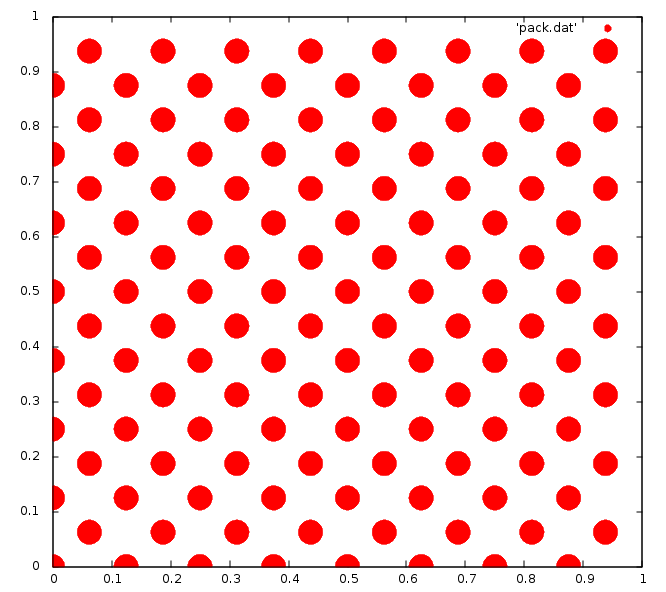
\includegraphics[scale=0.5]{sfere2D/reticolo.png}
	\caption{Disposizione iniziale dei dischi, $n=128$}
\end{figure}
Il reticolo che viene generato dipende solo dal numero di particelle utilizzate, la frazione di impacchettamento $\eta$ influisce solo sul diametro $\sigma$ dei dischi. Esso è dato da:
$$
	\sigma = \sqrt{\frac{4 \eta}{ \pi n}}
$$
La frazione di impacchettamento massima con questo reticolo è facilmente calcolabile, notando che ci sono due dischi per ogni cella reticolare (di lato $l$) :
$$
	\eta_max = \frac{ 2 A_{disco}}{A_{cella}} = \frac{2 \pi r_{max}^2}{l^2} = \frac{2 \pi (\sqrt{2} \frac{l}{4})^2}{l^2} = \frac{\pi}{4} = 0.7853982..
$$
Infine, si utilizzano condizioni di periodicità sui bordi della scatola in modi che il sistema abbia invarianza traslazionale.\\
Le velocità vengono inizializzate inizialmente in modo pseudocasuale con una distribuzione di velocità piatta compresa fra $[-1,1]$ e in seguito si impone che la velocità del centro di massa sia nulla.\\
Inoltre, si fissa la temperatura a 1, che equivale a fissare l'energia cinetica del sistema.
Questa è anche l'unica scala di energia del sistema, in quanto non c'è una scala di energia potenziale (esso vale $0$ o $\infty$).\\
La raccolta dati è stata effettuata per una durata di 15 unità di tempo\footnote{In unità di misura adimensionali} . Ciò significa che il numero di collisioni effettuate non è costante, ma cresce con la frazione di impacchettamento, siccome diminuisce il tempo di collisione medio:
\begin{center}

\begin{tabular}{c c}
\toprule
	$\eta$ & Numero collisioni \\
	\midrule
	0.2 & $\sim$ 27500 \\
	0.34 & $\sim$ 50000 \\
	0.56 & $\sim$ 123500 \\
	0.66 & $\sim$ 211000 \\
	0.75 & $\sim$ 335000 \\
	\bottomrule
\end{tabular}
\end{center}

\subsection{Termalizzazione}
Il sistema viene fatto termalizzare per 10000 collisioni prima di prendere dati.
Si è verificato che il sistema avesse termalizzato dopo questo numero di collisioni studiando la distribuzione di probabilità del modulo della velocità.\\
\begin{figure}[ht]
	\centering
	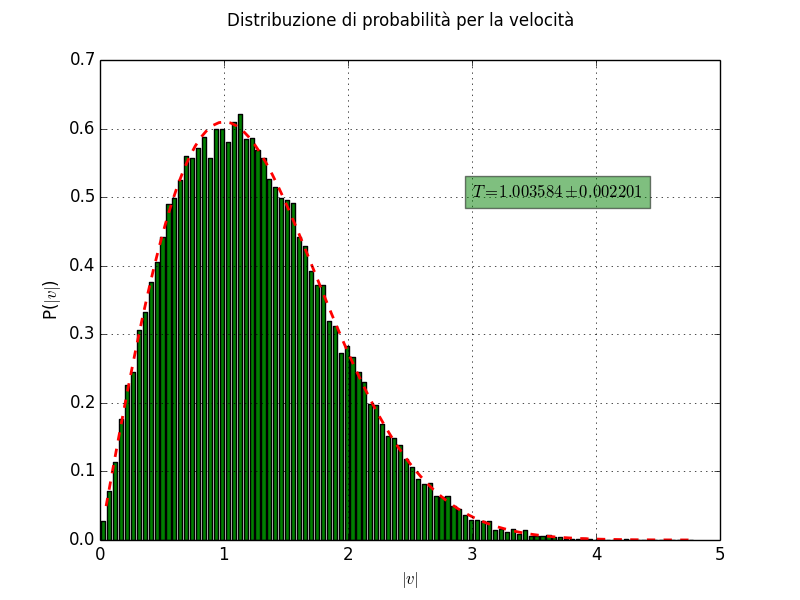
\includegraphics[scale=0.5]{sfere2D/boltzmann.png}
\end{figure}

Per fare ciò si è fatto partire il programma 400 volte, inizializzando il sistema sempre alla stessa temperatura e si è fatto un istogramma delle velocità calcolate dopo il ciclo di termalizzazione.
Si è poi fatto un fit con la distribuzione di Boltzmann in 2 dimensioni che è della forma:
$$
	P(|v|) = \frac{m}{k T} |v| e^{ - \frac{|v|^2}{2 k T}} = \frac{1}{T} |v| e^{ - \frac{|v|^2}{2T}}
$$
dove l'ultima uguaglianza vale per le unità di misura adimensionate che abbiamo utilizzato.\\
Il fit è stato fatto con la temperatura come unico parametro libero e concorda con la temperatura a cui è stato inizializzato il sistema:
$$
	T_{fit} = 1.003 \pm 0.002
$$


\subsection{Pressione}
Si analizza ora la pressione in funzione della frazione di impacchettamento.\\
Si è rappresentata la seguente osservabile, calcolata attraverso la formula\footnote{Utilizzata in unità di misura adimensionate: $V=1$,$k=1$,$m=1$}
\begin{center}
$$
	\frac{P V_0}{n k_{b} T} \, =\,  \frac{PV}{nT}\frac{\eta}{\eta_0} \, = 1 + \frac{m \sigma}{3 K_{en} t_{tot}} \sum_{coll} | \Delta v_{ij}| 
$$
\end{center}


Gli errori sono stato calcolati facendo girare dieci volte il programma agli stessi valori della frazione di impacchettamento e assegnando come errore la deviazione standard della media di questo campione di misure.

\begin{figure}[h!]
	\centering
	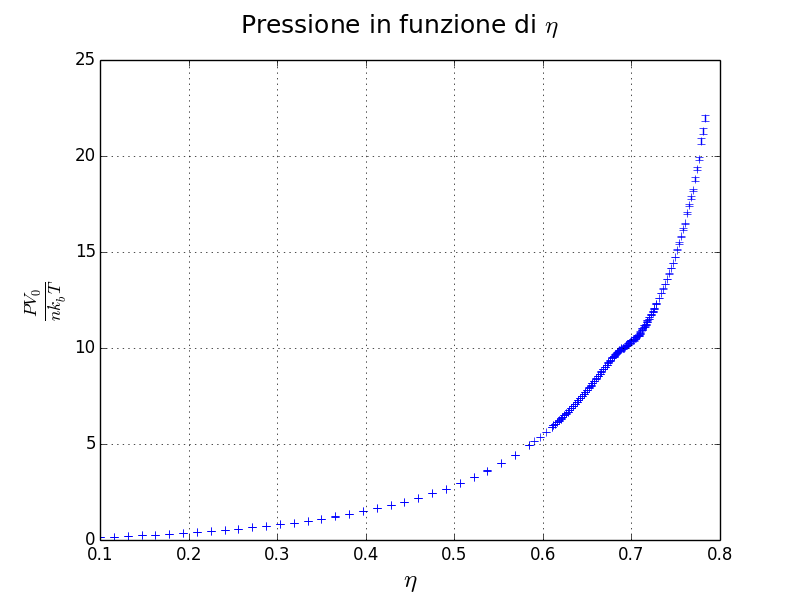
\includegraphics[scale=0.48]{sfere2D/pression.png}
	\caption{ $\frac{P V_0}{n k_{b} T}$ in funzione di $\eta$ con $n=128$ particelle}
	\end{figure}

\begin{figure}[h!]
	\centering
	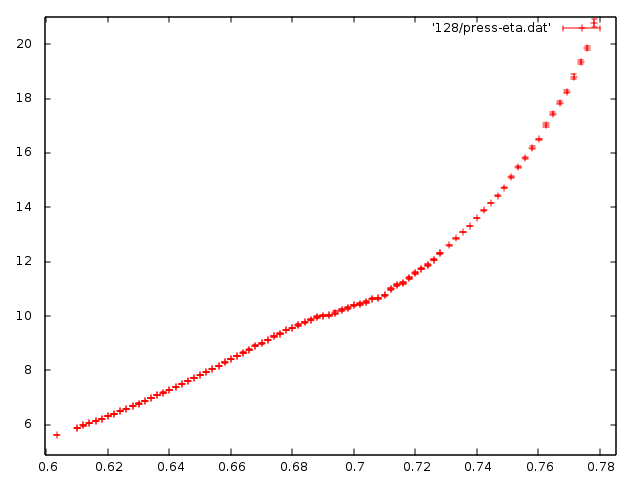
\includegraphics[scale=0.48]{sfere2D/pressionzoom.png}
	\caption{Ingradimento di $\frac{P V_0}{n k_{b} T}$ in funzione di $\eta$ con $n=128$ particelle}
	\end{figure}

\begin{figure}[h!]
	\centering
	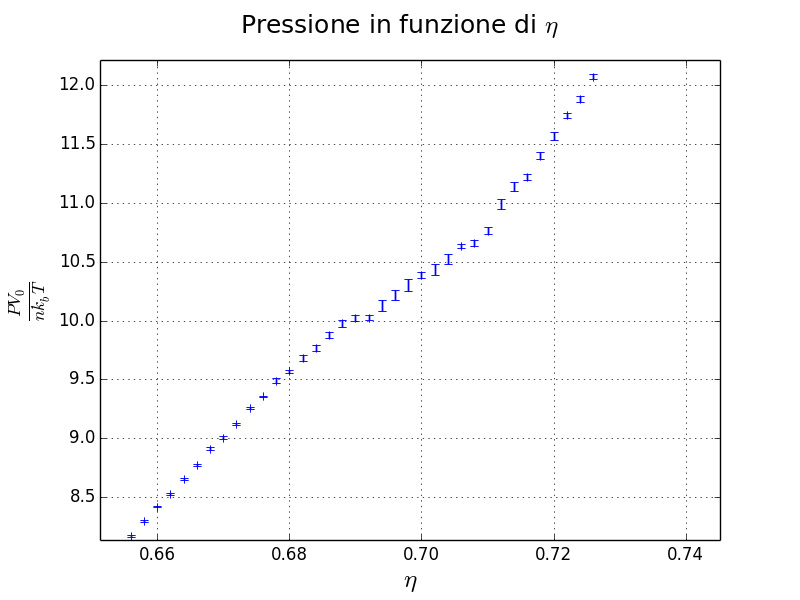
\includegraphics[scale=0.48]{sfere2D/pressionzoomzoom.png}
	\caption{Ulteriore ingrandimento di  $\frac{P V_0}{n k_{b} T}$ in funzione di $\eta$ con $n=128$ particelle}
	\end{figure}





Si può vedere dal grafico che questo sistema presenta una transizione di fase dovuta all'alta densità di impacchettamento.\\
La transizione inizia ad un valor della frazione di impacchettamento leggermente inferiore a $\eta \sim 0.69$, ma è presente una regione metastabile in cui la pendenza della curva si riduce notevolmente rispetto alla regione a frazione d'impacchettamento minore..
Subito dopo questo valore la curva ricomincia a salire, anche se con pe	ndenza minore.
Per $\eta \sim 0.71$ la pendenza della curva torna ad essere piatta, mentre per $\eta \sim 0.71$ la curva ricomincia a salire, con una pendenza superiore rispetto a prima della transizione di fase.\\
Le due regioni in cui la pendenza della curva si annulla sono agli estremi della regione in cui avviene la transizione di fase.\\
Superata la transizione di fase la pressione sale con una pendenza maggiore rispetto alla fase \emph{liquida}, altro segno che la stato del sistema è cambiato.


%%%%%%%%%%%%%%%%%%%%%%%%%%%%%%%%%%%%%%%%%%%%%%%%% RIGUARDAAAAAAAAAAAAAAAAAAAAAAAAAAAAAA%%%%%%%%%%%%%%%%%%%%%%%%%%

\subsection{Tempi di collisioni}

Come si è visto analizzando il numero di collisioni avvenute in funzione della frazione di impacchettamento, il tempo medio di collisione aumenta all'aumentare della frazione di impacchettamento.\\
Ciò è dovuto sostanzialmente al fatto che la distanza media tra il bordo dei dischi diminuisce all'aumentare del diametro e la distribuzione di velocità è pressochè simile al variare della frazione di impacchettamento.
Possiamo osservare questo comportamento sia analizzando il tempo di collisione medio tra i dischi sia studiando la distribuzione di probabilità associata ai tempi di collisione.\\

\subsubsection*{Tempo medio di collisione}
La quantità che è stata misurata è il tempo medio di collisione per particella. \'E stato calcolato usando la formula seguente:
$$
	t_{coll}  = \frac{t_{tot}}{2 N_{collisioni}} n_{particelle}
$$

Esso è stato calcolato per ogni simulazione e come nel caso della pressione, sono state ripetute 10 volte le misure. Da questo campione di dati si è calcolato media e deviazione standard della media.


\begin{figure}[h!]
	\centering
	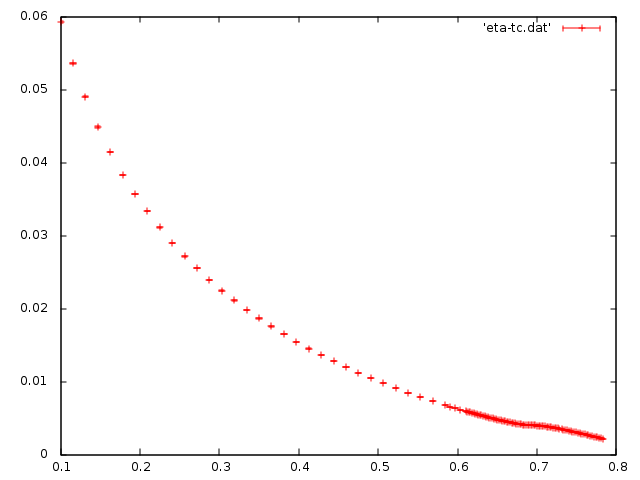
\includegraphics[scale=0.48]{sfere2D/tc.png}
	\caption{Tempo medio di collisione in funzione della funzione di impacchettamento, $n=128$}
	\end{figure}

\begin{figure}[h!]
	\centering
	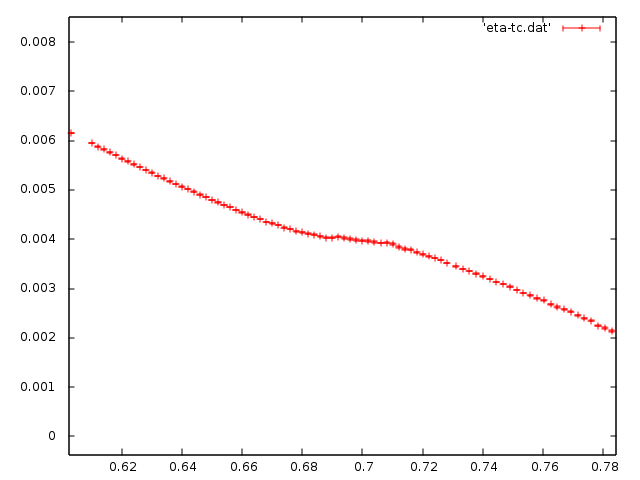
\includegraphics[scale=0.48]{sfere2D/tczoom.png}
	\caption{Ingrandimento del tempo medio di collisione in funzione della funzione di impacchettamento, $n=128$}
	\end{figure}

\begin{figure}[h!]
	\centering
	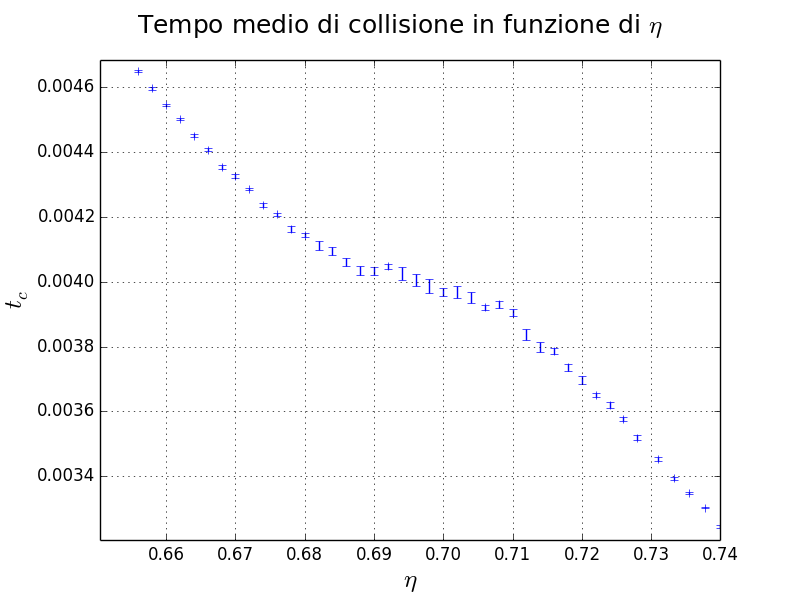
\includegraphics[scale=0.48]{sfere2D/tczoomzoom.png}
	\caption{Ulteriore ingrandimento del tempo medio di collisione in funzione della funzione di impacchettamento, $n=128$}
	\end{figure}



Come si può vedere dal grafico si ha una regione in cui la curva è quasi piatta a partire da un valore della frazione di impacchettamento poco sotto $\eta \sim 0.69$ fino a $\eta \sim 0.71$.\\
Questi sono gli stessi valori per cui si è notato un comportamento diverso della pressione nel grafico precedente.\\
Come si vedrà in seguito, questo intervallo di temperature caratterizzerà tutte le quantità che analizzeremo.
 
\subsubsection{Distribuzione di probabilità tempi di collisione}
Oltre ad analizzare il valor medio del tempo di collisione per particella, si può studiare anche la sua distribuzione di probabilità durante ogni simulazione.\\
Analizzando gli istogrammi creati a partire dai tempi di collisione di ogni singolo urto si può vedere che la distribuzione di probabilità è della forma:
$$
	P(t) = \frac{1}{\tau} \, e^{-\frac{t}{\tau}} \qquad \mbox{Normalizzata}
$$ 
dove $\tau$ si dimostrerà essere proprio il tempo di collisione medio per particella.\\
Ci si aspetta dunque che la distribuzione di probabilità diventi sempre più piccata aumentando $\eta$ (in quanto $t_{coll}$ diminuisce all'aumentare di $\eta$).
Si veda il caso per qualche valore di $\eta$:
\begin{center}
	\begin{figure}[h]
	\centering
		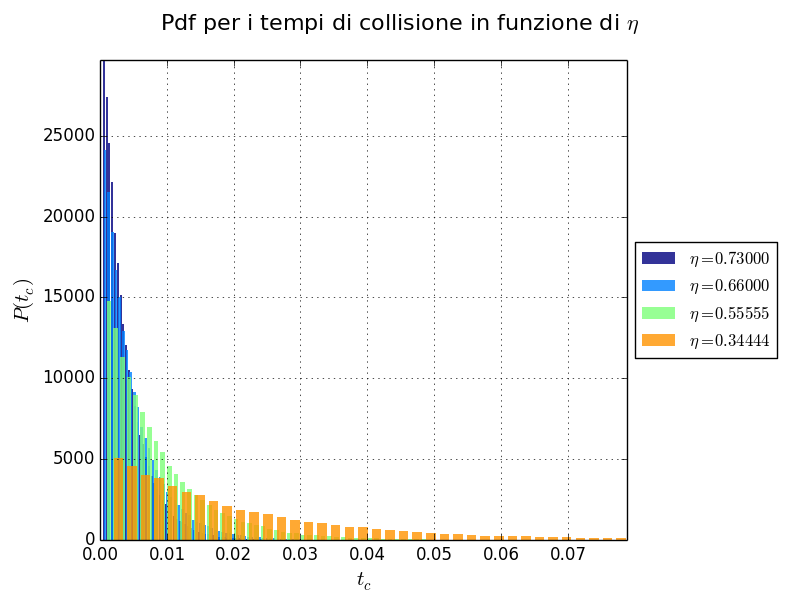
\includegraphics[scale=0.5]{sfere2D/pdf_tc.png}
	\caption{Confronto tra distribuzioni di probabilità per il tempo di collisione per particella a vari $\eta$}
	\end{figure}
\end{center}

Si veda inoltre il risultato del fit di uno di questi istogrammi con la distribuzione di probabilità citata sopra:

\begin{center}
	\begin{figure}[h!]
	\centering
		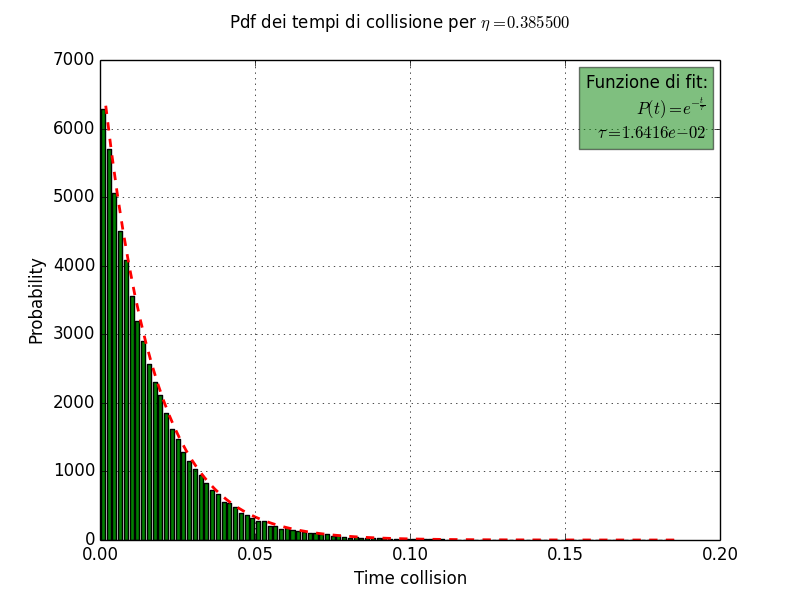
\includegraphics[scale=0.5]{sfere2D/fit_pdf_tc.png}
		\caption{Fit della distribuzione di probabilità con $e^{-\frac{t}{\tau}}$.}
	\end{figure}
\end{center}
Ci aspetta che il valore di $\tau$ ottenuto tramite questo fit coincida con il valor medio del tempo di collisione per particella calcolato durante l'esecuzione del programma. Si può capire ciò da questo semplice fatto:
$$
	<t> \, = \, \frac{1}{\tau}\int_0^{\infty} t \, e^{-\frac{t}{\tau}}\,dt = \tau
$$
Ci si aspetta quindi che se la distribuzione di probabilità è di quella forma allora il risultato del fit deve coincidere con il valor medio del tempo di collisione.\\
Nel grafico seguente si sono sovrapposti i valori di $t_{coll}$ calcolato come valor medio del tempo di collisione per particella e il valore di $\tau$ calcolati attraverso il fit:
\begin{center}
	\begin{figure}[h!]
		\centering
		\subfigure[Andamento generale]{
		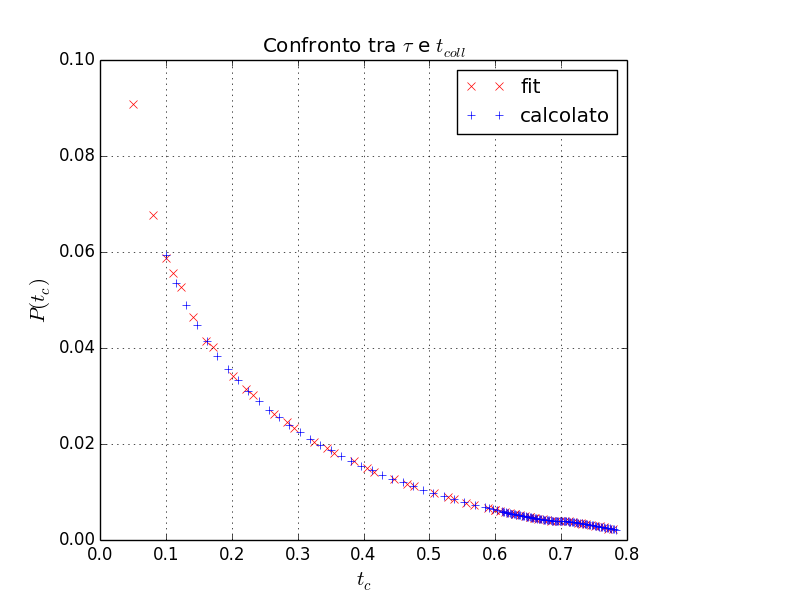
\includegraphics[scale=0.5]{sfere2D/tau_tcoll.png}
		}
		\subfigure[Ingradimento zona di transizione]{
		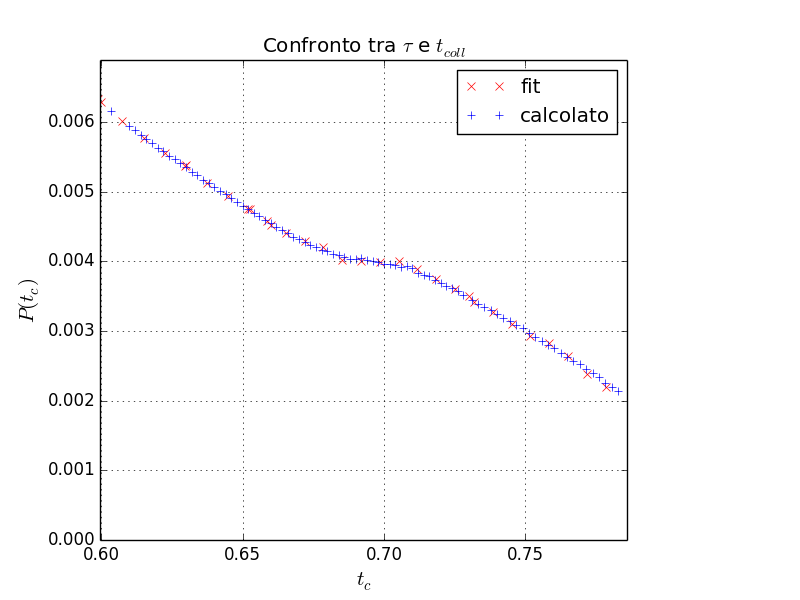
\includegraphics[scale=0.5]{sfere2D/tau_tcollzoom.png}
		}
	\caption{Confronto tra $t_{coll}$ e $\tau$}
	\end{figure}
\end{center}
Nel grafico non sono stati inseriti gli errori in quanto non sono stati calcolati gli errori associati agli istogrammi e quindi l'errore restituito dal fit non è del tutto significativo.\\
Si può vedere come l'accordo tra i due metodi di calcolo sia eccellente, anche nella regione di transizione di fase.
Ciò è segno del fatto che la distribuzione di probabilità mantenga sempre la forma $e^{-\frac{t}{\tau}}$ .




%%%%%%%%%%%%%%%%%%%%%%%%%%%%%%%%%%%%%%%%%%%%%%%%%%%%%%%%%%%%%%%%%%%%%%%%%%%%%%%%%%%%%%%%%%%%%%%%%%%%%%%%%%%%%%%%%%%%%%%%%%%%%%%%%%%%%%%%%%%%%%%%%%%%%%
\subsection{Libero cammino medio}
Il valore del libero cammino è stato calcolato mediando il libero cammino medio per particella fra tutte le particelle. Sono state eseguite 10 simulazioni come per le altre quantità e gli errori stato calcolati sulla base di questo campione.\\

\begin{figure}[h!]
	\centering
	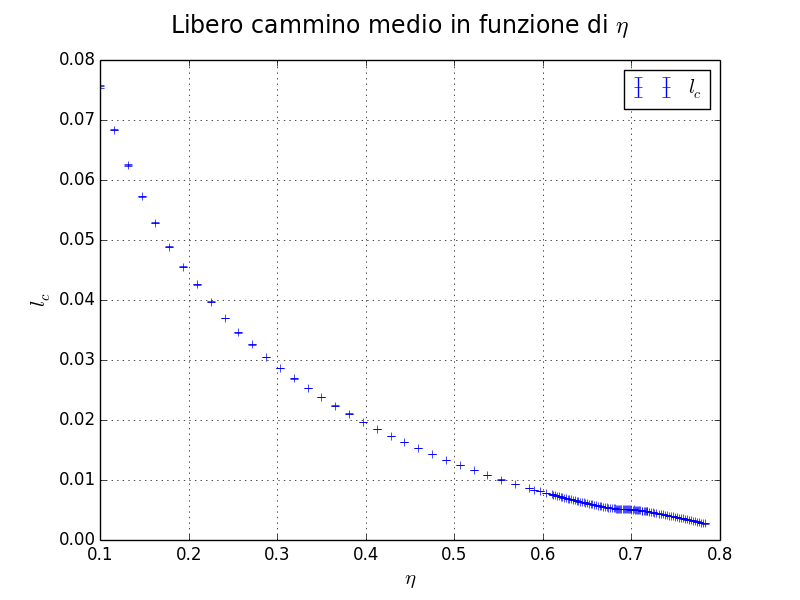
\includegraphics[scale=0.48]{sfere2D/mfp.png}
	\caption{Libero cammino medio in funzione di $\eta$}
	\end{figure}

\begin{figure}[h!]
	\centering
	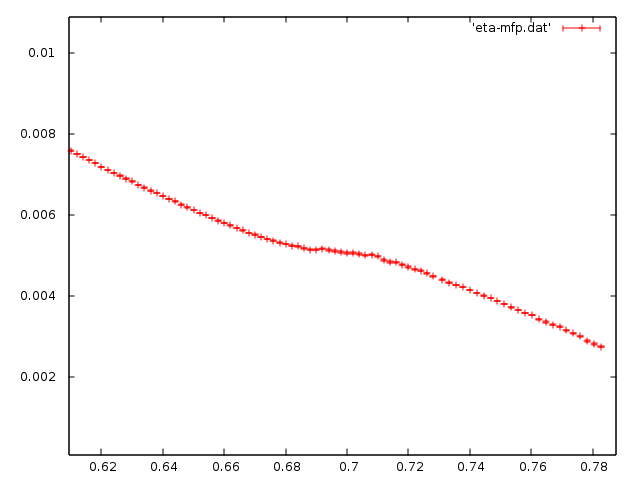
\includegraphics[scale=0.48]{sfere2D/mfpzoom.png}
	\caption{Ingrandimento del libero cammino medio in funzione di $\eta$}
	\end{figure}

\begin{figure}[h!]
	\centering
	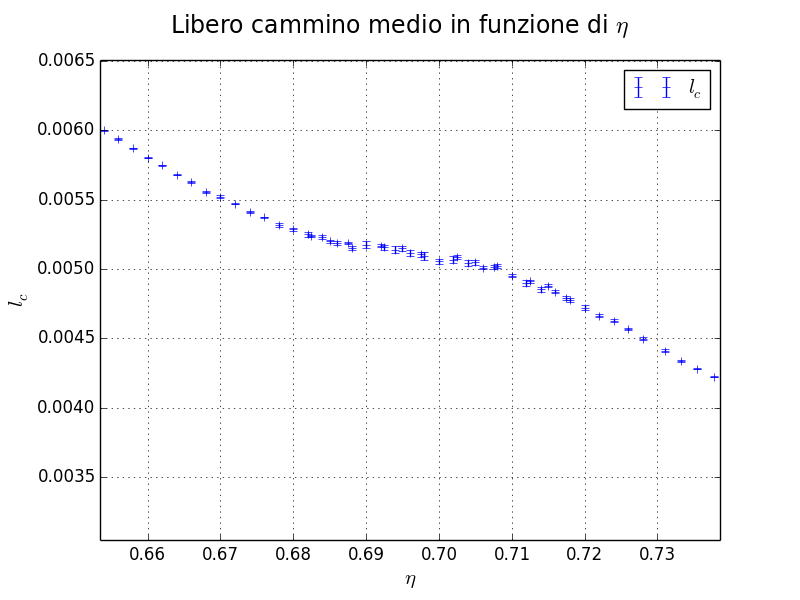
\includegraphics[scale=0.48]{sfere2D/mfpzoomzoom.png}
	\caption{Ulteriore ingrandimento del ibero cammino medio in funzione di $\eta$}
	\end{figure}

Si vede un comportamento del tutto simile a quanto accade con il tempo medio di collisione per particella, con una zona di transizione di fase nello stesso range di $\eta$ delle altre quantità.


\newpage
\subsection{Spostamento quadratico medio in funzione del tempo}
Il valore di $\Delta r^2(t)$ è stato calcolato per ogni singola particella, sfruttando l'invarianza temporale del sistema, mediando così tra tutti gli istanti distanti tra loro un tempo $t$. Infine, da questo campione di dati si è calcolato valor medio ed errore.\\
Il sistema è stato simulato fino a un valore del tempo pari a 15, ma i valori di $\Delta r^2(t)$ per $t$ superiore a 10 sono stati scartati in quando tendevano ad oscillare in quanto per essi il campione di dati era minore.\\
Si è calcolata questa quantità ad istanti di tempo discreti pari a 0.03 e per fare ciò è stato necessario spezzare l'evoluzione temporale in modo da prendere dati per valori multipli di 0.03.\\
Il valore aspettato per un sistema disordinato, prima della transizione di fase, è calcolabile teoricamente assumendo che in un tempo abbastanza grande ogni particella abbia avuto l'oppportunità di spostarsi in tutta la scatola. Esso è calcolabile in questo modo:
$$
<\Delta r^2(t)> \overset{\mathit{t\rightarrow \infty}}{\simeq} \int_{-\frac{L}{2}}^{\frac{L}{2}} dx \int_{-\frac{L}{2}}^{\frac{L}{2}} x^2 + y^2 = \frac{L^2}{6} \overset{\mathit{L=1}}{=} 0.166666..
$$
\begin{center}
	\begin{figure}[h]
	\centering
		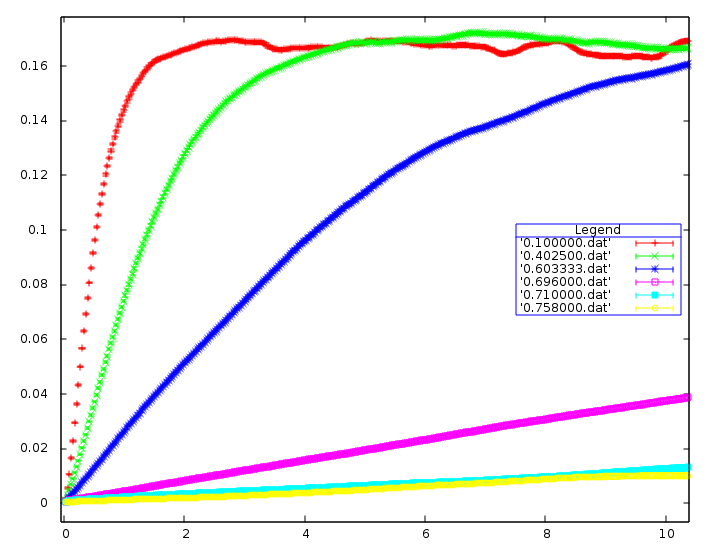
\includegraphics[scale=0.5]{sfere2D/dr2vari.png}
	\caption{Confronto tra i $\Delta r^2(t)$ a vari valori di $\eta$}
	\end{figure}
\end{center}
Come si può vedere dal grafico, per valori di $\eta$ non troppo vicini alla regione di transizione la curva arriva al valore teorico calcolato prima e poi si appiattisce. All'aumentare di $\eta$ la forma della curva cambia e diventa una retta in prima approssimazione, con una pendenza che decresce sempre più all'aumentare della frazione di impacchettamento. Questo comportamento è segno della scarsa mobilità dei dischi all'aumentare del loro diametro (ossia di $\eta$).
Per veder meglio questo fatto, si consideri il seguente grafico:
\begin{center}
	\begin{figure}[h!]
		\centering
		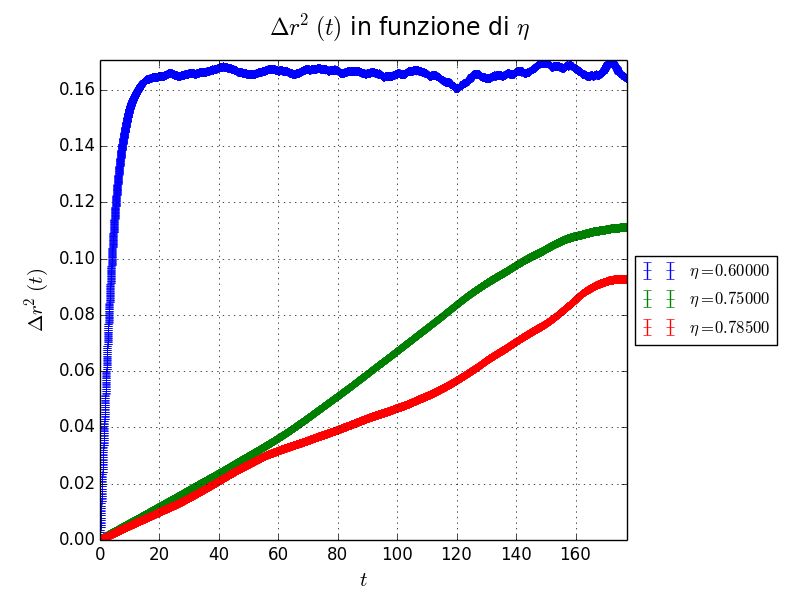
\includegraphics[scale=0.5]{sfere2D/dr2cfr.png}
	\end{figure}
\end{center}

Come si può vedere, prima della transizione di fase ($\eta=0.6$) il sistema arriva rapidamente al valore teorico e continua ad oscillare intorno a quel valore.
Per i valori successivi alla transizione di fase, le curve oltre ad avere una pendenza minore, esibiscono un comportamento diverso: non tendono più al valore calcolato teorico, calcolato nel caso di completa mobilità, ma si appiattiscono ad un altro valore, più basso.
Tale valore, come si può vedere, diminuisce all'aumentare di $\eta$, segno della sempre più scarsa mobilità dei dischi del sistema.
Da notare, inoltre, l'enorme tempo necessario per arrivare al valore limite, rispetto alla fase \emph{liquida}.


\newpage
\section{Sfere rigide 3D}

\subsection{Inizializzazione}
L'inizializzazione dell'algoritmo avviene in maniera del tutto simile a quanto fatto con i dischi in 2 dimensioni.
In questo caso, il reticolo in cui vengono inizializzate le particelle è un reticolo BCC. Per questo reticolo la cella elementare contiene 2 particelle.\\
La frazione di impacchettamento massima raggiungibile in questo caso è data da:
$$
	\eta_{max} = 2 \frac{V_{sfera}}{V_{cella}} = 2 \frac{ \frac{4}{3} \pi r_{max}^3}{ l^3 } = 2 \frac{\frac{4}{3} \pi
	( \frac{l \sqrt{3}}{4} )^3}{l^3 }= 0.6801747616....
$$
Le velocità sono state inizializzate come nel caso bidimensionale e anche la temperatura è stata fissata al valore 1.





\chapter{Sfere soffici}

\chapter{Modello di Ising}
Il modello è stato implementato su un reticolo bidimensione di larghezza N e inizializzando gli spin al valore $\pm 1 $  con uguale probabilità.
Sono stati implementati due algoritmi: Metropolis e Swendsen-Wang.\\

\section{Termalizzazione}
Possiamo valutare quando avviene la corretta termalizzazione del sistema analizzando l'andamento della magnetizzazione e dell'energia in funzione del tempo markoviano.
Di seguito è riportato l'andamento dell'energia e della magnetizzazione durante la termalizzazione a due diverse temperature.
\subsection*{Metropolis}
\begin{figure}[h]
\subfigure[$\beta=0.3$]{
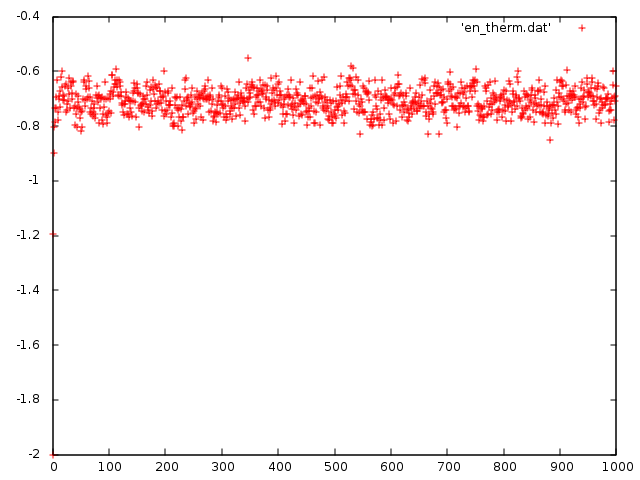
\includegraphics[scale=0.45]{metropolis/en_therm.png}
}
\subfigure[$\beta=0.453$]{
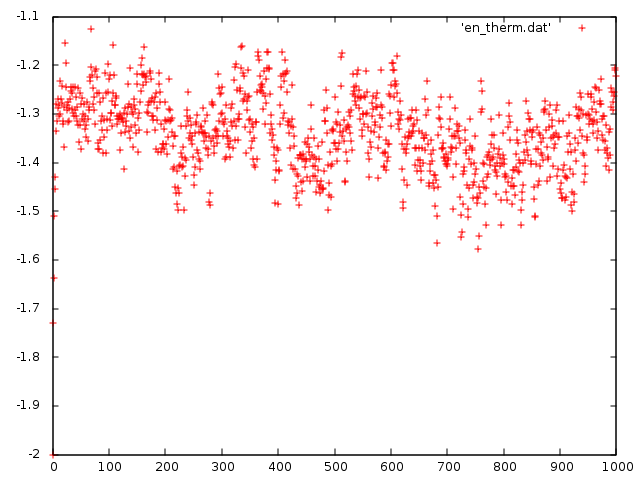
\includegraphics[scale=0.45]{metropolis/en_therm_crit.png}
}
\caption{Energia (Metropolis)}
\end{figure}
\begin{figure}[h]
\subfigure[$\beta=0.3$]{

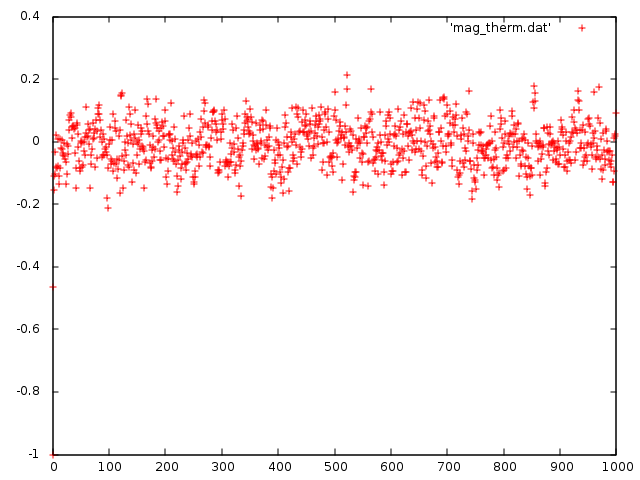
\includegraphics[scale=0.45]{metropolis/mag_therm.png}
}
\subfigure[$\beta=0.453$]{

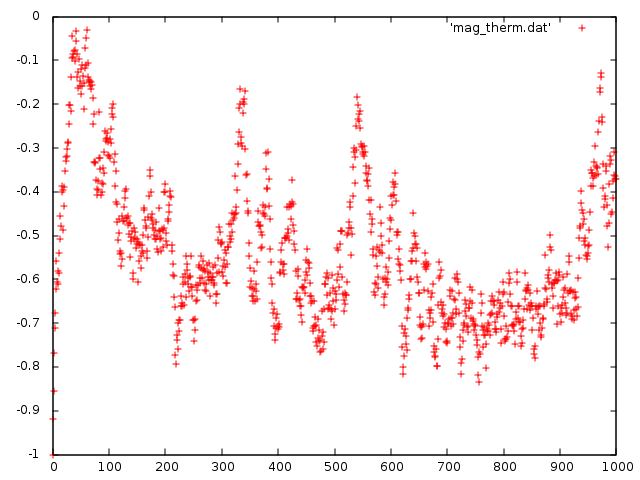
\includegraphics[scale=0.45]{metropolis/mag_therm_crit.png}
}
\caption{Magnetizzazione  (Metropolis)}
\end{figure}
Come si può vedere dal grafico relativo alla magnetizzazione a $\beta=0.453$, vicino al punto critico il tempo di termalizzazione cresce di molto. Esso rimane comunque intorno a 100 alla temperatura critica.
Dopo l'analisi di questi dati si è deciso di fissare il tempo di termalizzazione a 1000 passi temporali.
\subsection*{Swendsen-Wang}
\begin{figure}[h]
\subfigure[$\beta=0.3$]{
	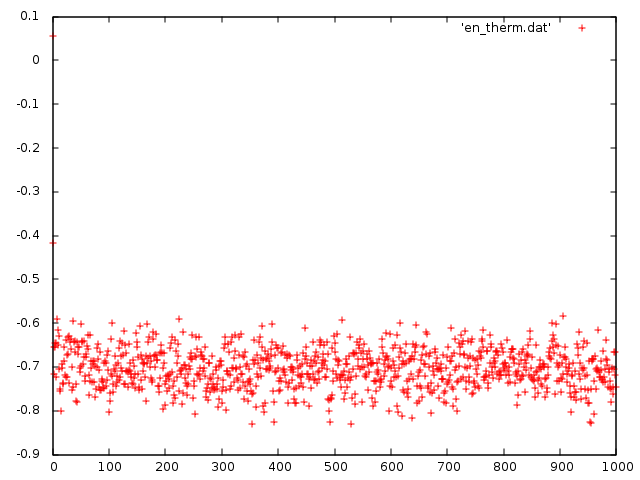
\includegraphics[scale=0.45]{sw/en_therm0-3.png}
}
\subfigure[$\beta=0.453$]{
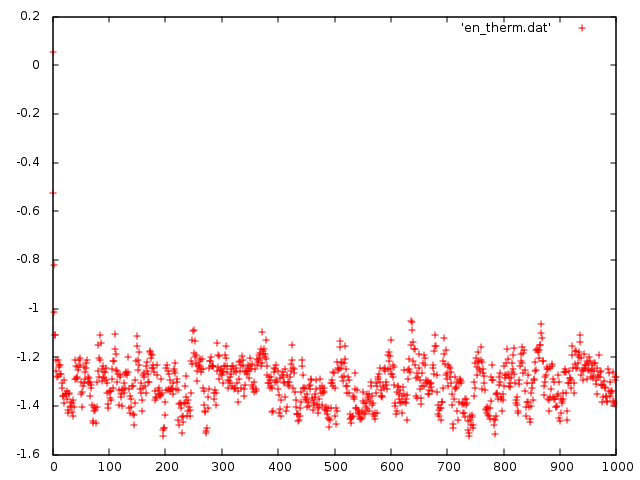
\includegraphics[scale=0.45]{sw/en_therm0-43.png}
}
\caption{Energia (Swendsen-Wang) }
\end{figure}

\begin{figure}[h]
\subfigure[$\beta=0.3$]{
	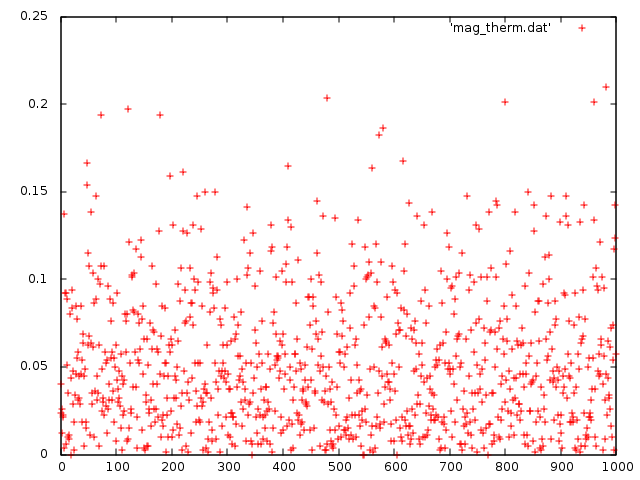
\includegraphics[scale=0.45]{sw/mag_therm0-3.png}
	}
\subfigure[$\beta=0.453$]{
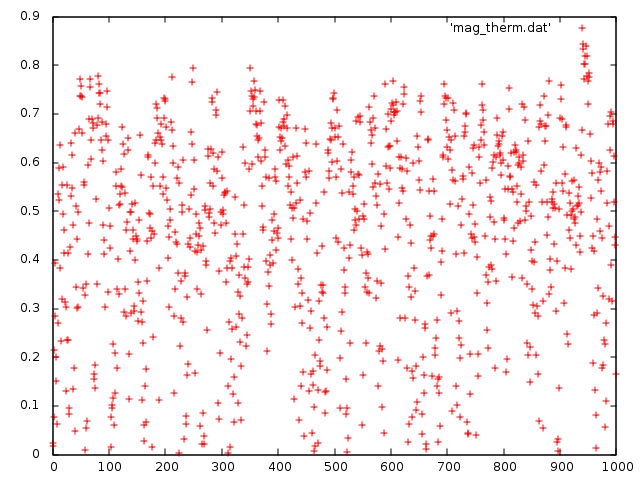
\includegraphics[scale=0.45]{sw/mag_therm0-43.png}
}
\caption{Magnetizzazione  (Swendsen-Wang)}
\end{figure}
Anche con questo algoritmo, il tempo di termalizzazione è molto minore dei 1000 passi utilizzati per far termalizzare il sistema nel programma.
La sostanziale differenza che si vede nei grafici relativi alla magnetizzazione vicino al punto critico è dovuta all'inefficienza dell'algoritmo Metropolis nell'estrarre configurazioni scorrelate vicino al punto critico, fenomeno solitamente chiamato \emph{critical slowing down}.
Esso si manifesterà più chiaramente nello studio dell'autocorrelazione delle configurazioni.


\section{Autocorrelazione fra le configurazioni}
Come in ogni simulazione Monte Carlo, è necessario studiare l'autocorrelazione delle configurazione estratte attraverso l'algoritmo in modo da stimare l'efficienza dell'algoritmo ad estrarre configurazioni
indipendenti e quindi nel produrre statistica.\\
Il tempo di autocorrelazione è stato calcolato utilizzando la formula:
$$
	\tau_{corr} = \frac{1}{2} + \sum_{t=1}^{t_{max}} \Gamma(t) \qquad \mbox{dove} \; \Gamma(t)= \frac{<f(x)f(x+t)> - <f(x)>^2}{<f^2(x)>-<f(x)>^2}
$$
\begin{figure}[h]
\centering
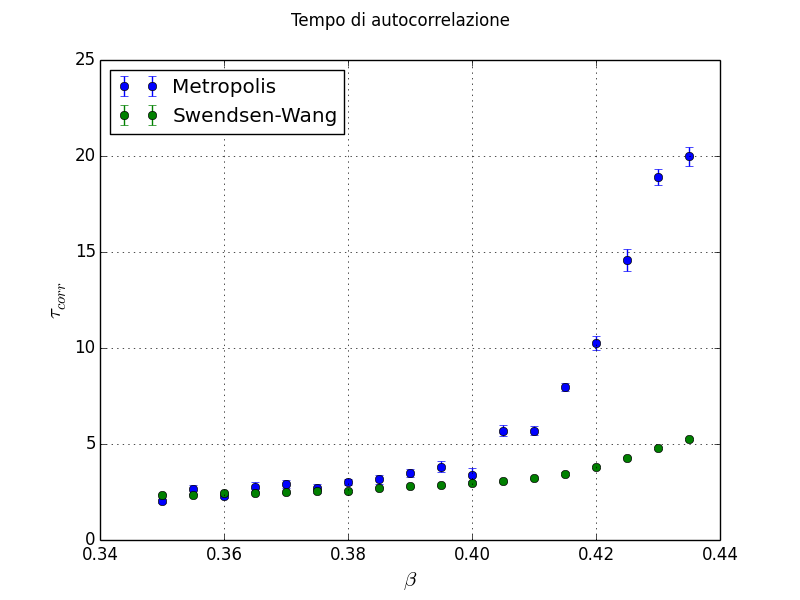
\includegraphics[scale=0.6]{compare.png}
\caption{Tempo di autocorrelazione dell'energia con N=46.}
\end{figure}
Gli errori sono stati stimati ripetendo le misure (in questo grafico 12 volte).\\
Inoltre, il valore di $ t_{max} $ è stato scelto pari a 60 in quanto per valori superiori le oscillazioni intorno a zero delle funzioni di autocorrelazione per valori di temperatura più lontani dal punto critico sono troppo rumorose e invalidano il calcolo di $\tau_{corr}$ per quei valori di temperatura. Infatti aumentando $t_{max}$ gli errori associati aumentavano molto, anche per i punti più vicini al punto critico.\\ 
Come si può vedere dai grafici, l'algoritmo Metropolis ha un tempo di autocorrelazione nettamente più elevato rispetto a Swendsen-Wang. Questo diverso comportamento è dovuto principalmente al fatto che Metropolis è un algoritmo locale, ossia l'inversione di ogni spin dipende esclusivamente dagli spin circostanti ad esso. L'algoritmo di Swendsen-Wang invece, è non-locale a causa della taglia estesa  che i cluster possono assumere.
Questo permette a questo algoritmo di non avere difficoltà ad estrarre configurazioni statisticamente scorrelate più velocemente rispetto a Metropolis.\\

Non è stato possibile stimare il valore di $\tau_{corr}$ per l'algoritmo Metropolis attraverso un fit con una funzione del tipo $e^{-\frac{t}{\tau_{c}}}$ in quanto vicino al punto critico l'autocorrezione smette di avere l'andamento esponenziale che ha lontano dal punto critico.\\
Ciò non accade, invece, per l'algoritmo Swendsen-Wang siccome l'autocorrelazione tra le configurazioni rimane piccola anche al punto critico.
Per questo algoritmo è stato possibile calcolare il tempo di autocorrelazione attraverso un fit per una grande range di temperature.
L'osservabile di cui si è calcolato l'autocorrelazione è l'energia.
Gli errori nel grafico sono quelli generati dal fit dell'esponenziale.

\begin{figure}
\centering
	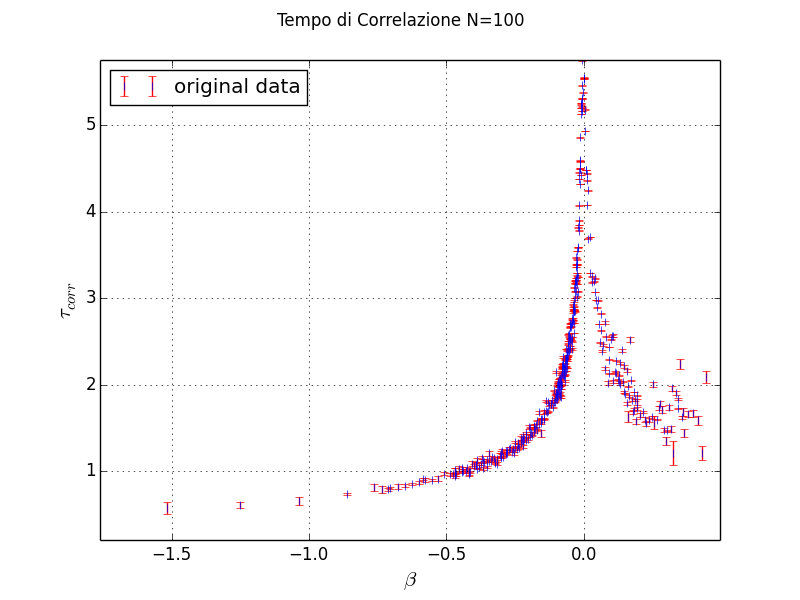
\includegraphics[scale=0.55]{sw/autocorrelazioneN100fit.png}
	\caption{Tempo di autocorrelazione con Swendsen-Wang tramite fit.}
\end{figure}
Il calcolo del tempo di autocorrelazione calcolato tramite fit concorda pienamente con l'altro metodo di calcolo.\\


\section{Binning}
Prima di affrontare la misura di osservabili è necessario analizzare come affrontare la correlazione fra le configurazioni estratte dagli algoritmi.
La tecnica migliore per ovviare a questo fatto è quella del \emph{binning}, ossia raggruppare misure in intervalli di larghezza abbastanza grande da diventare un gruppo di misure scorrelate tra loro.
A questo punto si procede a fare la media in ogni intervallo e si hanno così $\frac{N}{m}$ misure statisticamente indipendenti fra loro, a partire da $N$ misure autocorrelate suddivise in intervalli di larghezza $m$.\\
\'E fondamentale scegliere la larghezza corretta dell'intervallo. Ciò può essere fatto valutando l'andamento
della deviazione standard della media del nuovo set di $\frac{N}{m}$ misure in funzione di $m$.
Come si può immaginare, la larghezza del bin è associata al tempo di autocorellazione di cui si è parlato prima.

\subsection*{Metropolis}
Si vedano ora alcuni grafici di questa quantità a diverse temperature e per due diverse osservabili.
\begin{figure}[h!]
\subfigure[$\sigma$ Energia a $\beta=0.325$]{
	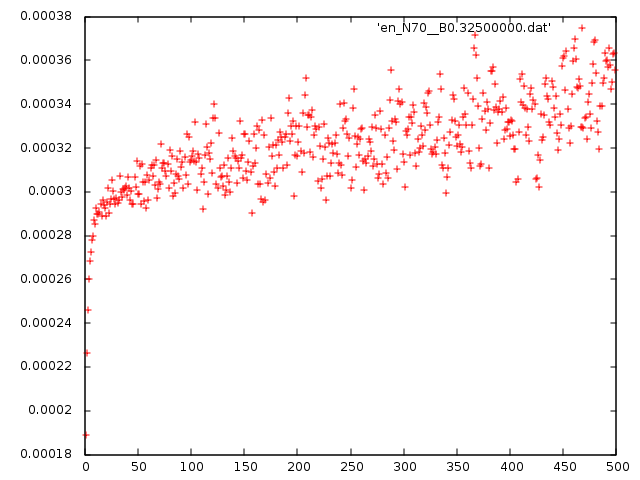
\includegraphics[scale=0.45]{metropolis/bin_en_0325.png}
}
\subfigure[$\sigma$ Energia $\beta=0.4508$]{
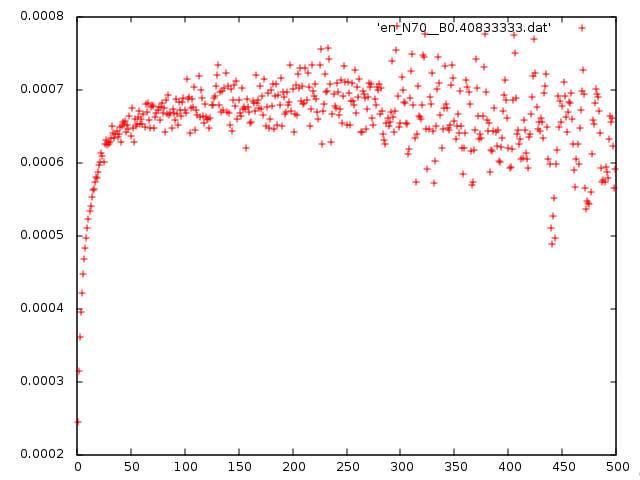
\includegraphics[scale=0.45]{metropolis/bin_en_0408.png}
}
\caption{Metropolis}
\end{figure}
\begin{figure}[h!]
\subfigure[$\sigma$ Energia a $\beta=0.453$]{
	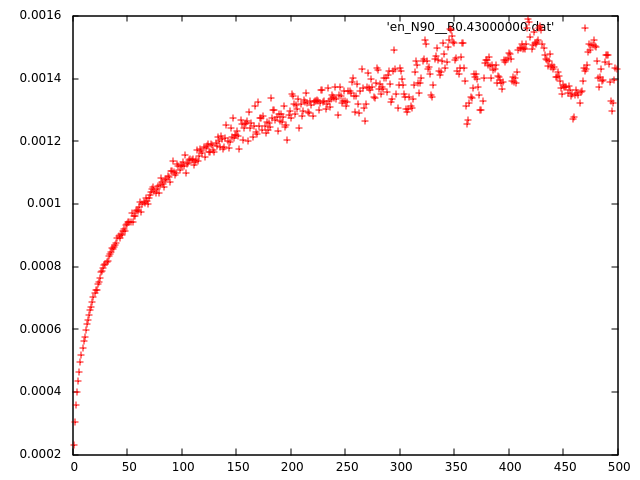
\includegraphics[scale=0.45]{metropolis/bin_en_043.png}
}
\subfigure[$\sigma$ Energia $\beta=0.459$]{
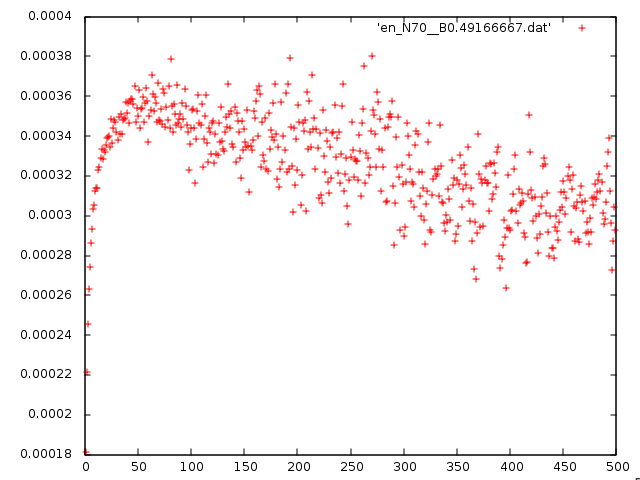
\includegraphics[scale=0.45]{metropolis/bin_en_049.png}
}
\caption{Metropolis}
\end{figure}

\begin{figure}[h!]
\subfigure[$\sigma$ Magnetizzazione a $\beta=0.325$]{
	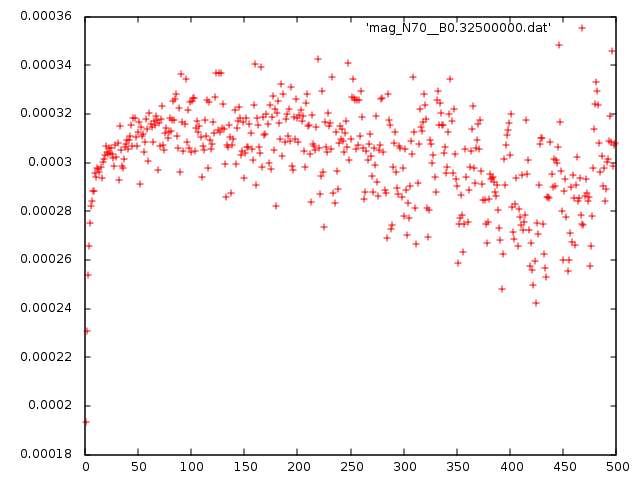
\includegraphics[scale=0.45]{metropolis/bin_mag_0325.png}
}
\subfigure[$\sigma$ Magnetizzazione $\beta=0.4508$]{
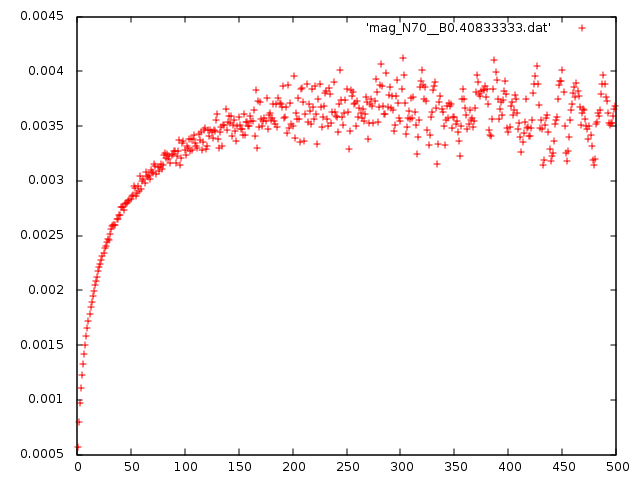
\includegraphics[scale=0.45]{metropolis/bin_mag_0408.png}
}
\caption{Metropolis}
\end{figure}
\begin{figure}[h!]
\subfigure[$\sigma$ Magnetizzazione a $\beta=0.43$]{
	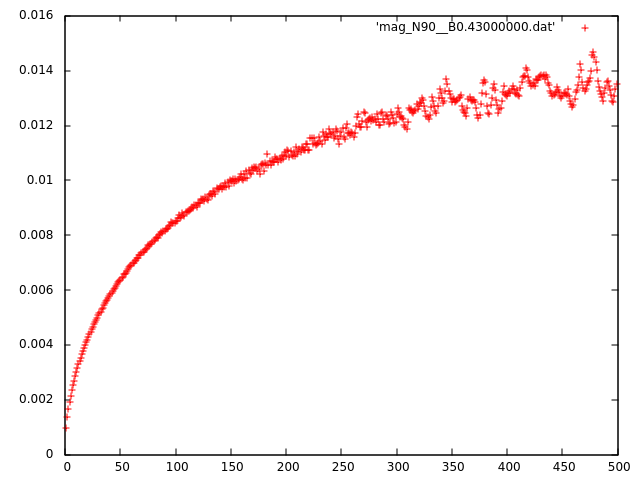
\includegraphics[scale=0.45]{metropolis/bin_mag_043.png}
}
\subfigure[$\sigma$ Magnetizzazione $\beta=0.49$]{
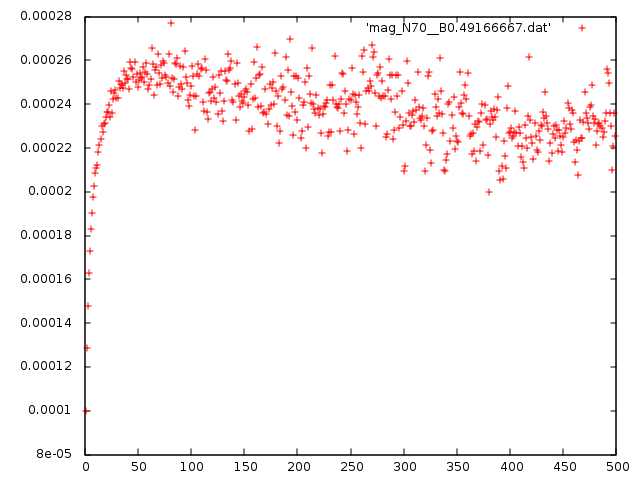
\includegraphics[scale=0.45]{metropolis/bin_mag_049.png}
}
\caption{Metropolis}
\end{figure}

\newpage
\subsection*{Swendsen-Wang}
Si vedano anche per questo algoritmo le stesse osservabili alle stesse temperature di Metropolis. 
\begin{figure}[h!]
\subfigure[$\sigma$ Energia a $\beta=0.325$]{
	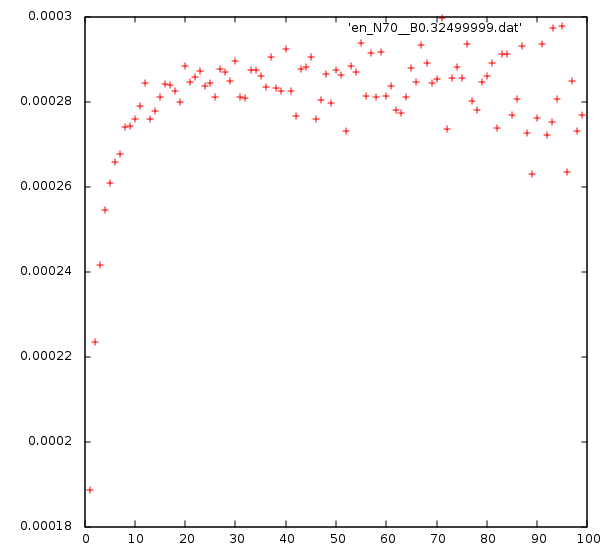
\includegraphics[scale=0.45]{sw/bin_en_0325.png}
}
\subfigure[$\sigma$ Energia $\beta=0.4508$]{
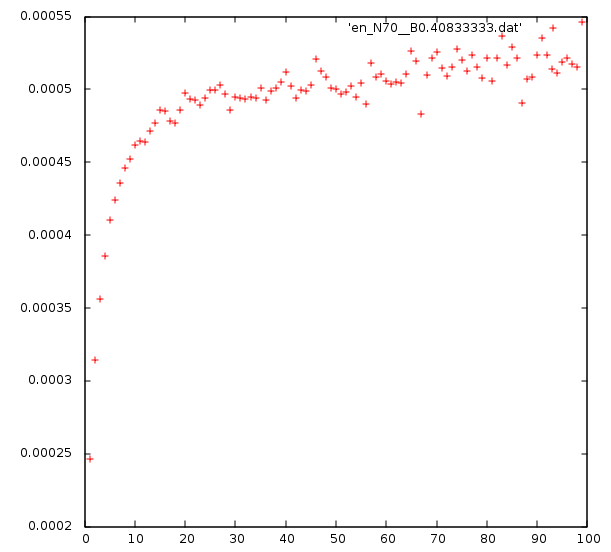
\includegraphics[scale=0.45]{sw/bin_en_0408.png}
}
\caption{Swendsen-Wang}
\end{figure}
\begin{figure}[h!]
\subfigure[$\sigma$ Energia a $\beta=0.453$]{
	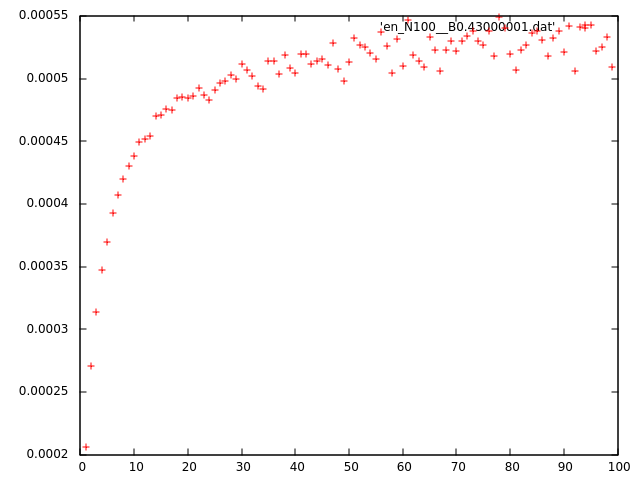
\includegraphics[scale=0.45]{sw/bin_en_043.png}
}
\subfigure[$\sigma$ Energia $\beta=0.459$]{
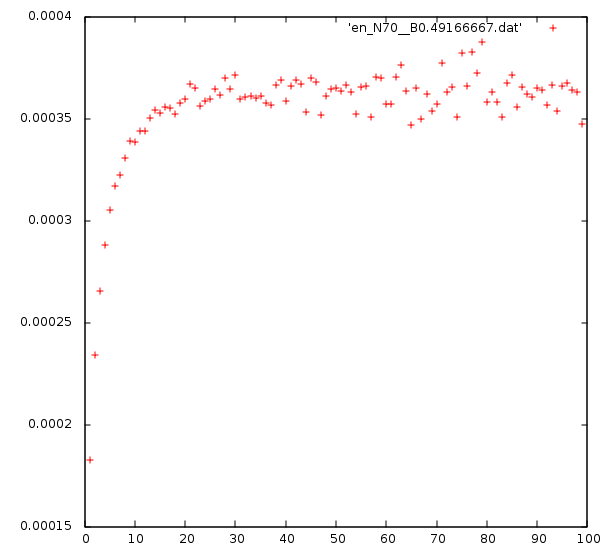
\includegraphics[scale=0.45]{sw/bin_en_049.png}
}
\caption{Swendsen-Wang}
\end{figure}


\begin{figure}[h!]
\subfigure[$\sigma$ Magnetizzazione a $\beta=0.325$]{
	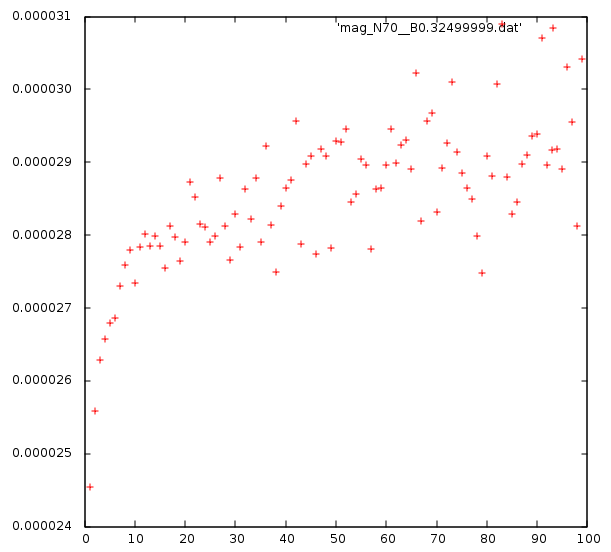
\includegraphics[scale=0.45]{sw/bin_mag_0325.png}
}
\subfigure[$\sigma$ Magnetizzazione $\beta=0.4508$]{
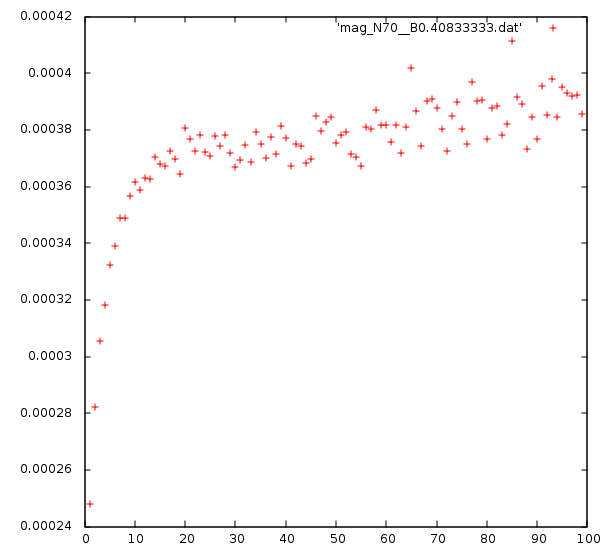
\includegraphics[scale=0.45]{sw/bin_mag_0408.png}
}
\caption{Swendsen-Wang}
\end{figure}
\begin{figure}[h!]
\subfigure[$\sigma$ Magnetizzazione a $\beta=0.43$]{
	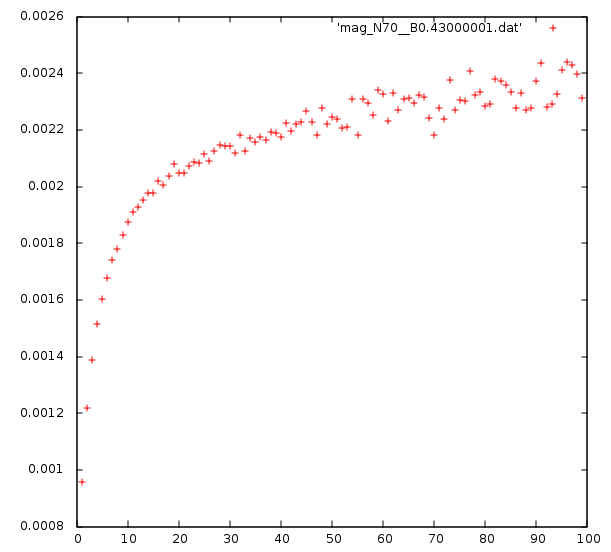
\includegraphics[scale=0.45]{sw/bin_mag_043.png}
}
\subfigure[$\sigma$ Magnetizzazione $\beta=0.49$]{
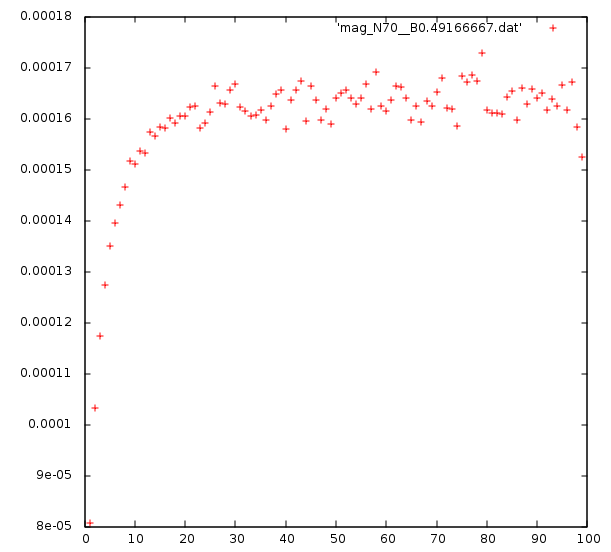
\includegraphics[scale=0.45]{sw/bin_mag_049.png}
}
\caption{Swendsen-Wang}
\end{figure}

Come si può vedere da un confronto diretto dei grafici, analizzando il valore per cui la curva di appiattisce, si può notare che, come ci si poteva aspettare, nell'algoritmo Metropolis è necessario scegliere una larghezza dell'intervallo molto alta vicino al punto critico, addirittura un ordine di grandezza superiore rispetto a Swendsen-Wang.
Si stima la larghezza ottimale dell'intervallo cercando il punto in cui la curva si appiattisce o inizia ad avere una derivata prima molto più piccola rispetto ai punti iniziali.
Si può vedere inoltre, come avvicinandosi al punto critico sia necessario avere un intervallo più largo: ciò è una chiara conseguenza della crescita di $\tau_{corr}$ all'avvicinarsi al punto critico.\\
Inoltre, prendiamo l'esempio del caso metropolis. Alla temperatura $\beta = 0.325$ possiamo prendere come larghezza del bin 20. Poco sotto il punto critico, avremo come larghezza bin ~ 150/200. Come nel caso dell'autocorrelazione avvicinandosi del punto critico la quantità in questione è aumentata di circa un fattore 10 in entrambi i casi.
Ciò può far capire perchè tempo di autocorrelazione e larghezza del bin siano due quantità non indipendenti.\\
A riprova di ciò, si può fare la stessa analisi con Swendsen-Wang: si passa da un larghezza del bin di circa 10 a una larghezza di circa 20. Esso è aumentato di un fattore simile al tempo di autocorrelazione, che è passato da 2.5 a 5.5 .\\
In seguito a questa analisi è stata scelta come larghezza dei bin per Metropolis  200 e per Swendsen-Wang 30.\\
Per via di questa grande differenza di larghezza dei bin il numero di passi temporali eseguiti con Metropolis è stato aumentato a 120000, mentre Swendsen-Wang rimane con 20000 passi in modo da avere errori più simili con i due algoritmi. In questo modo infatti si ha un numero di misure molto simile dopo il binning.\\
Nonostante Metropolis sia molto più veloce di Swendsen-Wang a parità di step temporali, la grande autocorrelazione fra le configurazioni generate impone di dover generare molte più configurazioni. Questo fatto lo rende più lento di Swendsen-Wang a generare un sample di dati simili.\\
Si confrontino i tempi dei due algoritmi in un reticolo 100x100:
\\
\begin{center}
\begin{tabular}{cc}
\toprule
	Metropolis (120000 step) & Swendsen-Wang (20000 step) \\
\midrule
	111 s & 48 s \\
\bottomrule
\end{tabular} 
\end{center}

L'algoritmo Swendsen-Wang risulta così più efficiente di Metropolis.
\newpage

\section{Energia e Magnetizzazione}
Energia e magnetizzazione sono le due principali osservabili di questo modello ed è possibile confrontare facilmente il loro andamento con la soluzione teorica di Onsager (valida però per un reticolo di taglia infinita).
Per la magnetizzazione è stata utilizzata l'osservabile \emph{improved} per Swendsen-Wang, ossia la frazione degli spin nel cluster più grande.
Nonostante i grafici siano stati fatti con un reticolo 100x100 l'accordo con la previsione teorica è eccellente per entrambe le osservabili e con entrambi gli algoritmi.
Insieme ai dati raccolti è stata sovrapposta la soluzione analitica di Onsager per entrambe le osservabili.
Gli errori sono stati calcolati attraverso il binning delle osservabili.
\begin{figure}[h]
	\subfigure[Metropolis]{
		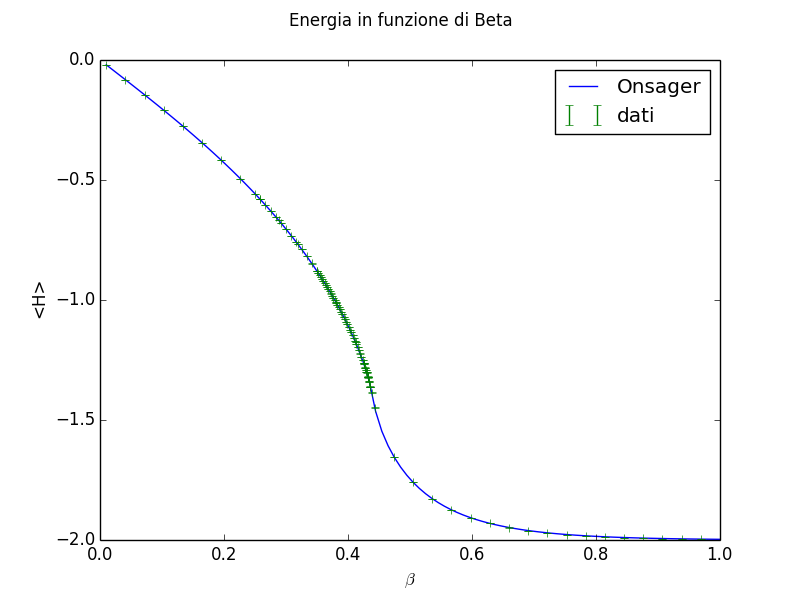
\includegraphics[scale=0.35]{metropolis/en_beta.png}
	}
	\subfigure[Swendsen-Wang]{
		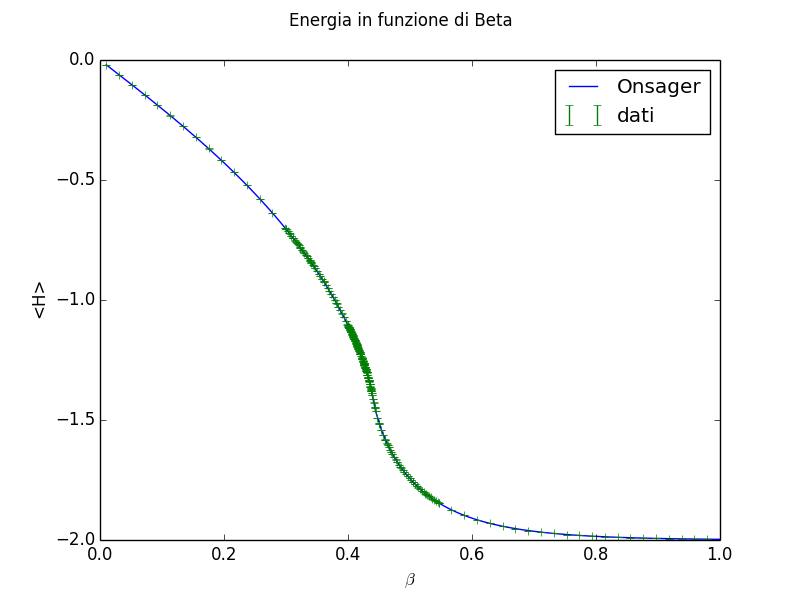
\includegraphics[scale=0.35]{sw/en_beta.png}
	}
\caption{Energia in funzione di $\beta$, 100x100.}
\end{figure}
Come si vede dai grafici, con entrambi gli algoritmi l'energia del sistema è perfettamente compatibile con la soluzione analitica già con un reticolo 100x100 e non si vedono differenze tra i due algoritmi.
\begin{figure}[h]
	\subfigure[Metropolis]{
		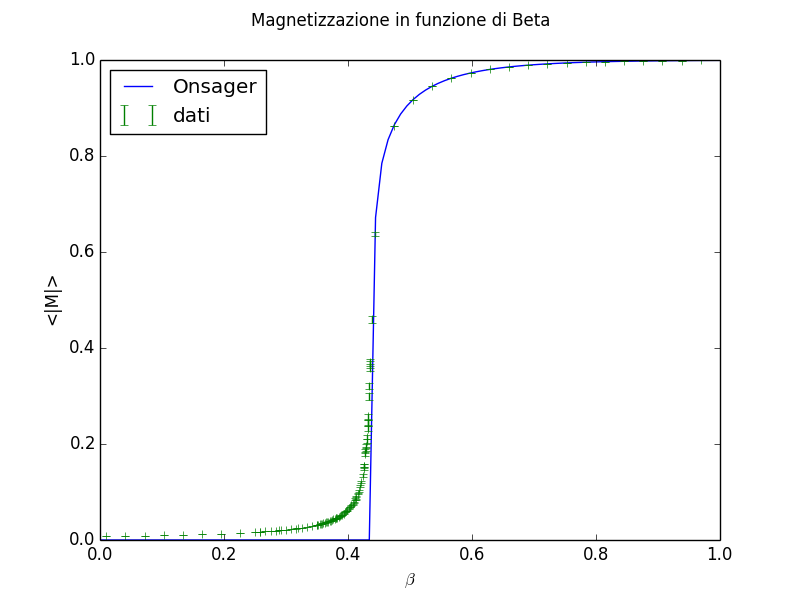
\includegraphics[scale=0.35]{metropolis/mag100.png}
	}
	\subfigure[Swendsen-Wang]{
		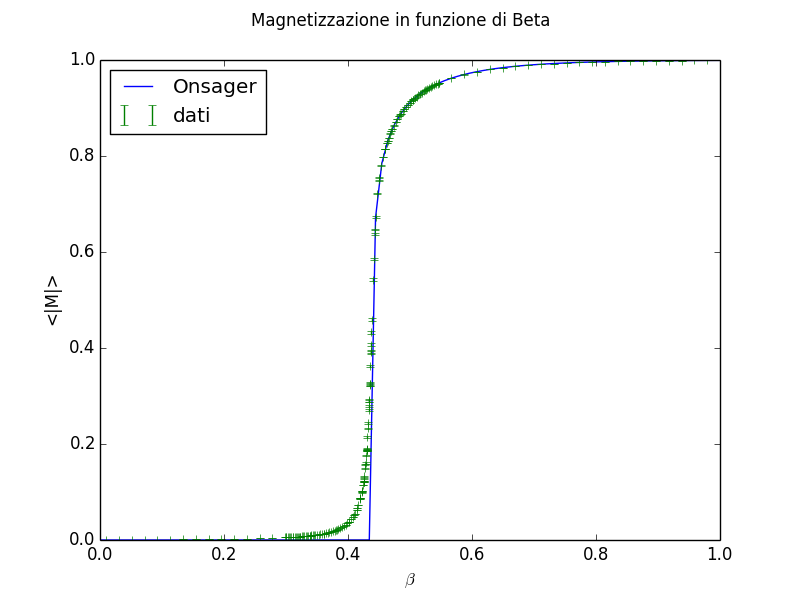
\includegraphics[scale=0.35]{sw/mag100.png}
	}
\caption{Magnetizzazione in funzione di $\beta$, 100x100.}

\end{figure}
\begin{center}
	\begin{figure}[h]
		\centering

		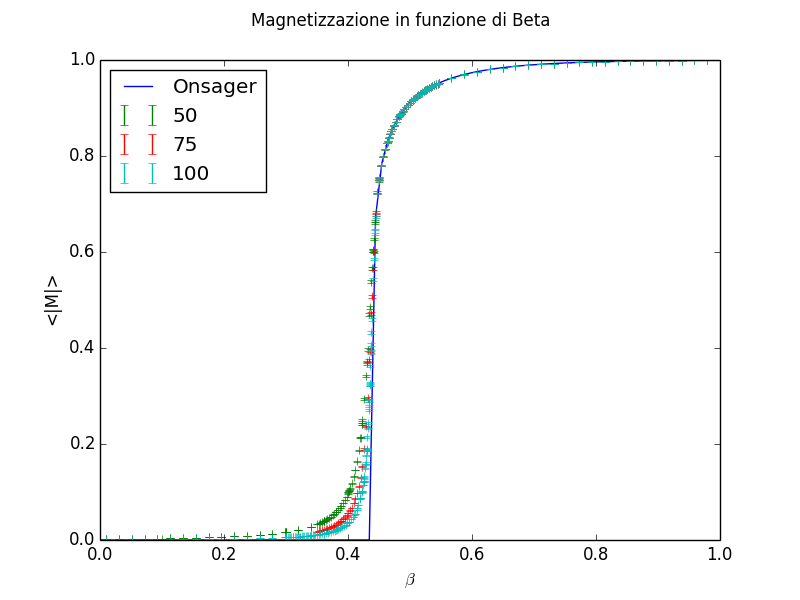
\includegraphics[scale=0.5]{sw/mag50100150.png}
		\caption{Magnetizzazione per L=50,75,100. Swendsen-Wang}
	\end{figure}
\end{center}

Diverso, invece, è il comportamento dei due algoritmi per la magnetizzazione. La differenza in questo caso è dovuto al fatto che per l'algoritmo Swendsen-Wang abbiamo utilizzato l'osservabile \emph{improved} ossia la frazione di siti nel cluster più grande.
Nella fase ferromagnetica i due risultati coincidono entrambi con la previsione teorica, mentre nella fase paramagnetica essi hanno un comportamento diverso fra di loro per il motivo appena spiegato, ma soprattutto diverso dalla soluzione teorica. \\
Ciò è da ricercare nella taglia finita del reticolo: infatti, per un sistema con un numero finito di gradi di libertà avremo che le osservabili sono sempre funzioni derivabili rispetto alla temperatura.
Solo nel limite termodinamico (e quindi con infiniti gradi di libertà) avremo osservabili non derivabili, come la magnetizzazione, e divergenti, come calore specifico e suscettività.
Per tutte queste osservabili per un numero finito di gradi di libertà avremo sempre funzioni lisce prive di divergenze, come si vedrà successivamente.\\
A sostegno di questa tesi si veda come all'aumentare della taglia del reticolo, la curva della magnetizzazione si avvicina sempre più a quella analitica, rimanendo sempre una funzione \emph{liscia}.

\section{Distribuzione di probabilità della magnetizzazione}

\begin{figure}[h]
\centering
	\subfigure[ $\beta=0.3$]{
		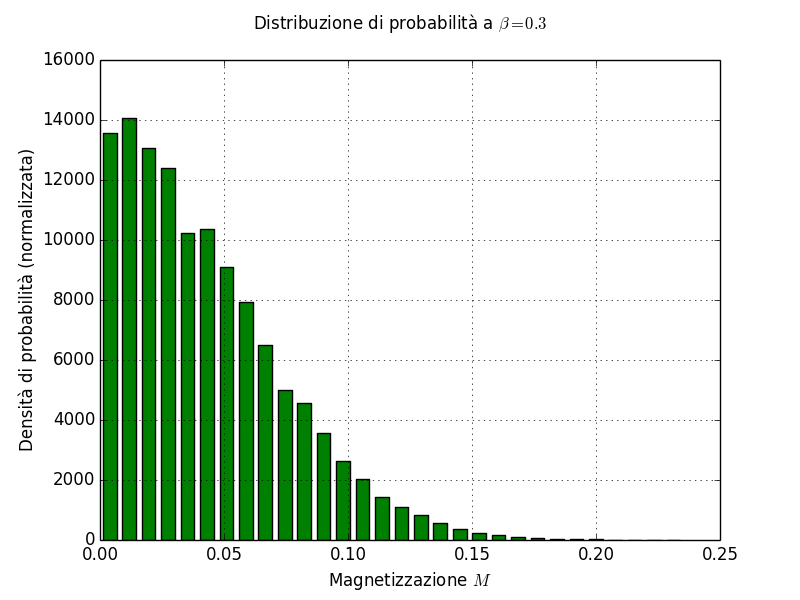
\includegraphics[scale=0.33]{metropolis/PDFM03.png}	
	}
	\subfigure[ $\beta=0.42$]{
		\includegraphics[scale=0.33]{metropolis/PDFM042.png}	
	}

	\caption{Metropolis}
\end{figure}
\begin{figure}[h]
\centering
		\subfigure[ $\beta=0.43$]{
		\includegraphics[scale=0.33]{metropolis/PDFM043.png}	
	}
	\subfigure[ $\beta=0.44$]{
		\includegraphics[scale=0.33]{metropolis/PDFM044.png}	
	}

	\caption{Metropolis}
\end{figure}

\begin{figure}[h]
\centering
		\subfigure[ $\beta=0.46$]{
		\includegraphics[scale=0.33]{metropolis/PDFM046.png}	
	}
	\subfigure[ $\beta=1$]{
		\includegraphics[scale=0.33]{metropolis/PDFM1.png}	
	}
	\caption{Metropolis}
\end{figure}

\begin{figure}[h]
\centering
	\subfigure[ $\beta=0.3$]{
		\includegraphics[scale=0.33]{sw/pdfM03.png}	
	}
	\subfigure[ $\beta=0.42$]{
		\includegraphics[scale=0.33]{sw/pdfM042.png}	
	}

	\caption{Swendsen-Wang}
\end{figure}
\begin{figure}[h]
\centering
		\subfigure[ $\beta=0.43$]{
		\includegraphics[scale=0.33]{sw/pdfM043.png}	
	}
	\subfigure[ $\beta=0.46$]{
		\includegraphics[scale=0.33]{sw/pdfM046.png}	
	}

	\caption{Swendsen-Wang}
\end{figure}

\begin{figure}[h]
\centering
	\subfigure[ $\beta=1$]{
		\includegraphics[scale=0.33]{sw/pdfM1.png}	
	}
	\subfigure[ $\beta=0.44$]{
		\includegraphics[scale=	0.33]{sw/pdfM044.png}	
	}
	\caption{Swendsen-Wang}
\end{figure}
Si studia ora la distribuzione di probabilità del modulo della magnetizzazione al variare della temperatura, confrontando fra loro i due algoritmi in questione.
Si è deciso di studiare il modulo della magnetizzazione in quanto l'algoritmo Swendsen-Wang ad ogni step inverte i cluster (con probabilità $\frac{1}{2}$), mentre Metropolis, siccome inverte uno spin alla volta, tende a mantere costante il segno della magnetizzazione per temperature sotto il punto critico.\\
I grafici sono stati calcolati per un reticolo 50x50.

Come si vede dai grafici, essi sono molto simili tra i due algoritmi e le leggere differenze che si notano sono da imputare al fatto che, anche in questo caso, per la magnetizzazione in Swendsen-Wang è stata utilizzata l'osservabile \emph{improved}.\\
Da questi istogrammi inoltre, si vede chiaramente come l'avvicinarsi al punto critico comporti un allargamento della larghezza della distribuzione. Questo è prevedibile in quanto, a meno di un fattore di volume, la varianza della magnetizzazione è la suscettività magnetica che ha un massimo (per un sistema finito) al punto critico.\\
A fronte di questo fatto, si può anche stimare che la temperatura critica per il reticolo 50x50 (quello utilizzato per gli istogrammi) è inferiore a $\beta=0.44$, dato che a questa temperatura la magnetizzazione è già più piccata che a $\beta=0.43$.


\newpage

\section{Lunghezza di correlazione}
\begin{figure}[h]
\centering
	\includegraphics[scale=0.5]{metropolis/cor120.png}
\caption{Lunghezza di correlazione $L=120$:Metropolis}
\end{figure}


La lunghezza di correlazione è stata stimata dal calcolo di:
$$
	<S_0 S_t > \, = \, A \, e^{-\frac{t}{\xi}} \qquad \mbox{dove} \qquad S_n = \frac{1}{L} \sum_i \sigma_{(n,i)} 
$$
Nel calcolo di $<S_0 S_t>$, inoltre è stata sfrutta l'invarianza per traslazione, rotazione di $\frac{\pi}{2}$ e inversione del reticolo, in modo da diminuire l'errore associato a questa grandezza.
Si sfrutta l'invarianza per traslazione calcolando più precisamente la seguente quantità:
$$
	<S_0 S_t> = \frac{1}{L} \sum <S_i S_{t+i}>
$$ 

\begin{figure}[h]
\centering
	\includegraphics[scale=0.5]{sw/corrN120.png}
\caption{Lunghezza di correlazione $L=120$:Swendsen-Wang}
\end{figure}
L'invarianza per rotazioni di $\frac{\pi}{2}$ è stata utilizzata mediando il calcolo fra righe e colonne. Inoltre è stata utilizzata anche l'invarianza per inversione  e la ciclicità del reticolo, le quali insieme comportano la validità di questa relazione:
$$
	< S_0 S_t> = < S_0 S_{L-t}>
$$
A questo punto si è calcolata osservabile e si sono stimati gli errori attraverso un binning come per le altre osservabili.
I Valori della lunghezza di correlazione sono poi così stati stimati fittando con un esponenziale decrescente. I valori ottenuti dal fit (errori compresi) sono stati utilizzati per i grafici della lunghezza di correlazione in funzione della temperatura.\\
A questo punto si è confrontata la dipendenza della lunghezza di correlazione $\xi$ con la previsione teorica, che prevede una divergenza (per un reticolo infinito) a potenza per temperature vicine a quella critica:
\begin{align*}
	\xi \sim t^{-\nu} \qquad \mbox{per} \; t \sim 0 \qquad \mbox{con} \; \nu = 1 \; \mbox{(teorico)}  \\
	t = \frac{\beta - \beta_{crit}}{\beta_{crit}} \qquad \beta_{crit} = 0.4406868
\end{align*}
per il valore di temperatura critica è stato utilizzato quello teorico
Gli estremi dell'intervallo in cui è stato fatto il fit sono stati scelti in modo che la correlazione rimanesse un ordine di grandezza inferiore al lato del reticolo, per evitare che la taglia finita del reticolo influenzasse la misura dell'esponente. Inoltre, si è cercato di rimanere quanto più possibile vicini al punto critico visto che l'equazione sopra citata vale nell'intorno del punto critico.\\
Dopo queste considerazioni è stato scelto come intervallo per il fit i valori $[0.415,0.43]$ per entrambi gli algoritmi. Il valore massimo di lunghezza di correlazione che si ottiene è $\sim 22$ che è piccolo rispetto al lato del reticolo pari a $120$. 
Il risultato del fit è quindi:
\begin{center}
	\begin{tabular}{cc}
	\toprule
	Algoritmo & $\nu$ \\
	\midrule
	Metropolis & $ 1.004 \pm 0.009 $\\
	Swendsen-Wang	& $ 1.018 \pm 0.005 $\\
	\bottomrule
	\end{tabular}
\end{center}

Con entrambi gli algoritmi si sono ottenuti risultati compatibili tra loro e abbastanza vicini alla previsione teorica.\\
Bisogna tenere in considerazione che la taglia finita del reticolo incide su molti aspetti relativi al calcolo dell'esponente critico. Primo fra tuttti non è possibili avvicinarsi troppo al punto critico perchè la taglia finita del reticolo modifica la divergenza (teorica) e la rende finita. Oltre a questo, la temperatura critica per un reticolo finito è leggermente più bassa di quella teorica che è stata utilizzata per effettuare il fit. 
\newpage
\section{Finite Size Scaling}
\subsubsection*{Calcolo suscettività e calore specifico}
Per il calcolo di queste due osservabili non è stato utilizzato il binning nello stesso modo usato per energia e magnetizzazione. Questo perchè sono definite utilizzando i valori medi di energia e magnetizzazione.\\
Per questo motivo sono stati creati degli intervalli di larghezza 3000 invece che 30 e sono state eseguite 30000 iterazioni dell'algoritmo, per diminuire l'errore.\\
La formula utilizzata è la seguente:
\begin{align*}
	c = \frac{1}{V} < \mathcal{H}^2>_{bin} - <\mathcal{H}>_{bin}^2 \\
	\chi = V < \mathcal{M}^2>_{bin} - <\mathcal{M}>_{bin}^2
\end{align*}
dove con $< ..>_{bin}$ si intende il valor medio sul bin di larghezza 3000 di cui si è parlato.

\subsection*{Stima di $\beta_{crit}$ e Finite Size Scaling }

Si andranno ora a fare uno studio di \emph{finite size scaling} per poter valutare l'accordo dei dati ottenuti per magnetizzazione, suscettività e calore specifico con gli esponenti critici esatti della soluzione di Onsager.
Per fare uno studio di \emph{finite size scaling} è necessario raccogliere dati sulle osservabili in esame per varie taglie del reticolo. In questo caso sono state utilizzati i seguenti reticoli:
\begin{itemize}
\item 35x35 
\item 50x50 
\item 65x65
\item 90x90
\item 120x120 
\item 150x150
\end{itemize}

A questo punto, per suscettività e calore specifico è stato necessario calcolare per ogni taglia del reticolo  la temperatura critica.\\
Si è deciso di stimare la temperatura critica facendo un fit con una parabola e stimando la temperatura critica come il massimo della parabola. Ciò ha dato risultati soddisfacenti nel caso della suscettività, mentre per il calore specifico il fit con la parabola non stimava correttamente la temperatura critica.
Per questo motivo, si è deciso di utilizzare la temperatura critica stimata attraverso la suscettività per ciascuna taglia del reticolo anche per il calore specifico. \\
Così facendo si è trascurata la dipendenza della temperatura critica dall'osservabile.
A posteriori si può vedere come questa assunzione sia giustificata vedendo il grafico dopo aver effettuato il finite size scaling per questa osservabile.\\
Le temperature critiche trovate in funzione della taglia del reticolo sono le seguenti:
\begin{center}
	\begin{tabular}{c c}
	\toprule
	Reticolo & $\beta_{crit}$ \\
	\midrule
	35x35 &  0.430294 \\ % 0.430437
	50x50 &  0.433357 \\ %0.433357
	65x65 & 0.435147 \\ %0.435147
	90x90 & 0.436540\\
	120x120 & 0.437669 \\ %0.437669
	150x150 & 0.438262 \\
	\end{tabular}
\end{center}
Per questo dato non è stato calcolato l'errore associato in quanto avrebbe richiesto ripetere varie volte le misure e siccome questa misura serve solo per poter effettuare il finite size scaling in modo corretto, il suo errore non influenza il risultato del finite size scaling.
Per la magnetizzazione questo non è stato necessario in quanto non presenta alcun picco.\\
Dopo aver ricavato la temperatura critica, si fa una traslazione sulla temperatura portandola nella nuova variabile 
$$
	 t = \frac{\beta - \beta_{crit}}{\beta_{crit}}
$$ 
Infine si effettua l'ultimo scaling, indicando con $L$ la taglia del reticolo e considerando la magnetizzazione si avrà:
\begin{align*}
	t \longrightarrow L^{\frac{1}{\nu}} t = L t \\
	M \longrightarrow \frac{M}{L^{\frac{-\beta}{\nu}}} = \frac{M}{L^{-\beta}}
\end{align*}
Per la suscettività si avrà:
$$
	\chi \longrightarrow \frac{\chi}{L^{\frac{\gamma}{\nu}}} = \frac{\chi}{L^{\gamma}}
$$
Nel caso del calore specifico, la soluzione analitica prevede che abbia esponente $\alpha=0$ il che indica uno scaling di tipo logaritmo. Per esso l'equazione precedente viene modificata in:
$$
	c \longrightarrow \frac{c}{\log{L}}
$$
Gli esponenti critici della soluzione analitica sono i seguenti:\\
\begin{center}
	\begin{tabular}{c c }
		\toprule
		Esponente & valore \\
		\midrule
		$\alpha$ & 0 \\
		$\beta$ & $1/8$\\
		$\gamma$ & $7/4$ \\
		\bottomrule
	\end{tabular}
\end{center}
Essi sono stati utilizzati per effettuare gli scaling delle varie osservabili.
\begin{center}
	\begin{figure}[h]
		\centering
		\includegraphics[scale=0.6]{sw/fssmag.png}
		\includegraphics[scale=0.6]{sw/fssmagzoom.png}
		\caption{Studio di Fss per $M= t^{\beta}$, con $\beta=\frac{1}{8}$}
	\end{figure}
\end{center}
\begin{figure}[h]
		\centering
		\includegraphics[scale=0.6]{sw/fsschi.png}
		\includegraphics[scale=0.6]{sw/fsschizoom.png}
		\caption{Studio di Fss per $\chi = t^{-\gamma}$, con $\gamma = \frac{7}{4}$}
\end{figure}

\begin{center}
	\begin{figure}[h]
		\centering
		\includegraphics[scale=0.6]{sw/fsscv.png}
		\includegraphics[scale=0.6]{sw/fsscvzoom.png}
		\caption{Studio di Fss per $c = \log{ t} $ ( $\alpha=0$)}
	\end{figure}
\end{center}


A questo punto, ci si aspetta di vedere che le curve per ciascuna taglia, opportunamente scalate nella procedura descritta, collassino su un'unica curva \emph{universale}.
Come si può vedere dai grafici per queste tre osservabili è proprio ciò che accade nella regione paramagnetica con $\beta < \beta_{crit}$.\\
Siccome il \emph{finite size scaling} si basa sugli esponenti critici della soluzione esatta, dal risultato di questa analisi possiamo dire che le osservabili calcolate scalano in modo molto simile a ciò che ci si aspetterebbe teoricamente.
Per questo, gli esponenti critici del modello simulato sembrano risultare simili a quelli previsti teoricamente.

\newpage
\chapter{Modello di Potts}
Il modello di Potts è una generalizzazione del modello di Ising studiato nel capitolo precedente.
Esso generalizza il modello di Ising aggiungendo un numero arbitrario di stati.\\
 Si analizzerà ora il modello di Potts in 2 dimensioni con 3 stati. La sua implementazione ha sfruttato la rappresentazione degli stati come radici dell'unità $e^{2 \pi i}$ con $i=0,1,2$.
Il modello è stato implementato solo usando l'algoritmo Swendsen-Wang e verrà svolta un'analisi simile a quanto fatto con Ising data l'analogia tra i due modelli.


\section{Termalizzazione}

\begin{figure}[h!]
	\subfigure[$\beta=0.5$]{
		\includegraphics[scale=0.28]{potts/en_therm05.png}	
	}
	\subfigure[$\beta=1$]{
		\includegraphics[scale=0.28]{potts/en_therm1.png}	
	}
	\subfigure[$\beta=1.5$]{
		\includegraphics[scale=0.28]{potts/en_therm15.png}	
	}
	\caption{Andamento dell'energia in fase di termalizzazione}
\end{figure}

\begin{figure}[h!]
	\subfigure[$\beta=0.5$]{
		\includegraphics[scale=0.28]{potts/mag_therm05.png}	
	}
	\subfigure[$\beta=1$]{
		\includegraphics[scale=0.28]{potts/mag_therm1.png}	
	}
	\subfigure[$\beta=1.5$]{
		\includegraphics[scale=0.28]{potts/mag_therm15.png}	
	}
	\caption{Andamento della magnetizzazione in fase di termalizzazione}
\end{figure}
I siti del reticolo vengono inizializzati in modo uniformemente casuale tra i tre stati possibili.
Dopo aver analizzato l'andamento di energia e magnetizzazione nella fase di termalizzazione si è scelto di impostare un tempo di termalizzazione pari a 1000 passi temporali anche se come si può vedere dai grafici, già 100 passi sono sufficienti.

\section{Binning}
Il binning è stato implementato esattamente come nel modello di Ising. Siccome questo modello è stato simulato attraverso Swendsen-Wang ci si aspetta che la larghezza dei bin sia comparabile a quella nel modello di Ising con il medesimo algoritmo. Infatti così accade e anche in questo caso è stata scelta una larghezza degli intervalli pari a 30. Il numero totale di passi temporali dell'algoritmo è in questo caso di 10000, quindi si hanno circa la metà dei dati rispetto a Ising con Swendsen-Wang.\\
Si veda ora l'andamento della deviazione standar nel punto critico, temperatura in cui si ha l'autocorrelazione massima tra le configurazioni. A tutte le altre temperature, come nel modello di Ising, la curva si appiattisce molto più rapidamente.
\begin{center}
\begin{figure}[h!]
	\centering

 	\subfigure[ $\sigma$ della magnetizzazione]{
	\includegraphics[scale=0.4]{potts/mag_bincrit.png}
	}
 	\subfigure[ $\sigma$ dell'energia]{
	\includegraphics[scale=0.4]{potts/en_bincrit.png}
	}

\end{figure}
\end{center}

\section{Energia e Magnetizzazione}
A differenza del modello di Ising non si ha la soluzione analitica esatta di magnetizzazione ed energia in funzione della temperatura, quindi non è possibile confrontarle direttamente.\\
Si può vedere che la temperatura a cui avviene la transizione di fase è di poco sopra $\beta=1$ come previsto. I grafici sono stati fatti con un reticolo di taglia 100x100.
\begin{figure}[h!]
	\centering
	\includegraphics[scale=0.55]{potts/en100.png}
	\caption{Energia per $L=100$}
\end{figure}
\begin{figure}[h!]
	\centering
	\includegraphics[scale=0.55]{potts/mag100.png}
	\caption{Magnetizzazione (improved) per $L=100$}
\end{figure}
Come nel caso del modello Ising, si possono apprezzare le differenze fra le diverse taglie del reticolo osservando la curva di magnetizzazione nella fase paramagnetica, dove le curve sono molto diverse tra loro, a differenza della fase ferromagnetica in cui questa differenza sparisce.\\
Le curve sono relative a reticoli 30x30,75x75 e 150x150:

\begin{figure}[h]
\centering
\includegraphics[scale=0.5]{potts/mag_taglia.png}
\caption{Magnetizzazione per L=30,75,150.}
\end{figure}
\newpage
\section{Distribuzione di probabilità della magnetizzazione}
In questo modello, si può analizzare la distribuzione della probabilità della magnetizzazione nel piano complesso.
Ciò può essere fatto utilizzando la seguente definizione di magnetizzazione:
$$
	 M = \frac{| \sum_{siti} \phi_{i j} |}{N} 
$$
Se non si considera il modulo, essa può essere studiata nel piano complesso.\\
\begin{center}
\begin{figure}[h!]
\centering
 	\subfigure[$\beta=0.81$]{
	\includegraphics[scale=0.33]{potts/potts08.png}
	}
 	\subfigure[$\beta=0.9$]{
	\includegraphics[scale=0.33]{potts/potts09.png}
	}

 	\subfigure[$\beta=0.81$]{
	\includegraphics[scale=0.33]{potts/magmod081.png}
	}
 	\subfigure[$\beta=0.9$]{
	\includegraphics[scale=0.33]{potts/magmod09.png}
	}

\end{figure}
\end{center}
\begin{center}
\begin{figure}[h!]
\centering
 	\subfigure[$\beta=0.97$]{
	\includegraphics[scale=0.33]{potts/potts097.png}
	}
 	\subfigure[$\beta=0.99$]{
	\includegraphics[scale=0.33]{potts/potts099.png}
	}

 	\subfigure[$\beta=0.97$]{
	\includegraphics[scale=0.33]{potts/magmod097.png}
	}
 	\subfigure[$\beta=0.99$]{
	\includegraphics[scale=0.33]{potts/magmod099.png}
	}


\end{figure}
\end{center}


\begin{center}
\begin{figure}[h!]
\centering
	 	\subfigure[$\beta=1.005$]{
 	\includegraphics[scale=0.33]{potts/potts1005.png}
}
 	\subfigure[$\beta=1.015$]{
	\includegraphics[scale=0.33]{potts/potts1015.png}
	}
	 	\subfigure[$\beta=1.005$]{
 	\includegraphics[scale=0.33]{potts/magmod1005.png}
}
 	\subfigure[$\beta=1.015$]{
	\includegraphics[scale=0.33]{potts/magmod1015.png}
	}
\end{figure}
\end{center}


Come si vede dai grafici, quando si è vicini al punto critico e quindi la distribuzione di probabilità della magnetizzazione è molto larga, inizia ad emergere la figura di un triangolo che degenere nei 3 vertici superata la regione critica.\\
La comparsa di questi 3 punti è da imputare al tipo di algoritmo utilizzato per simulare questo modello, ossia Swendsen-Wang.
Ciò è infatti analogo a quanto accade al modello di Ising con il medesimo algoritmo se si studia la magnetizzazione senza aggiungere il modulo. Ciò è dovuto al fatto che ad ogni passo, per ogni cluster viene estratto un nuovo valore con probabilità $1/q$ dove $q$ è il numero di stati.\\
Per il modello di Potts con $q=4$, per esempio, otterremo i vertici di un quadrato e così via.


\newpage
\section{Lunghezza di correlazione}
Lo studio della lunghezza di correlazione è del tutto analago al modello di Ising.\\
La definizione dell'osservabile che permette di stimare la lunghezza di correlazione è diversa dal modello di ising:
$$
	Re(<S_0 S_t>) = A e^{-t \xi}
$$
Come nel modello di Ising è stata sfruttata l'invarianza per traslazioni, rotazioni e periodicità per diminuire l'errore associato a $<S_0 S_t>$.
Un altro commento necessario è relativo alla scelta dell'intervallo in cui fare il fit della lunghezza di correlazione.\\
Come nel caso di Ising, la temperatura più alta è scelta in modo che la lunghezza di correlazione sia molto minore rispetto alla taglia del reticolo, che in questo caso è 150x150. Anche in questo caso, l'estremo inferiore è stato scelto molto vicino al punto critico: l'intervallo è dunque il range di temperature $[0.95,0.995]$.
Anche in questo caso è stata utilizzata come valore di $\beta_{crit}$ quello teorico, ossia
$\beta_{crit} = log(1+\sqrt(3)) = 1.0050525..$
\begin{center}
\begin{figure}[h]
\centering
 	\includegraphics[scale=0.65]{potts/corr150.png}
 	\caption{Lunghezza di correlazione.}
\end{figure}
\end{center}

\begin{center}
\begin{tabular}{c c }

	\toprule
	metodo & valore \\
	\midrule
	teorico & $ 5/6 = 0.8333333 $ \\
	calcolato & $ 0.833 \pm 0.007 $\\

\end{tabular}

\end{center}


\newpage
\section{Finite Size Scaling}
Lo studio di finite size scaling per questo modello è del tutto analogo a quanto fatto con il modello di Ising, con l'unica differenza che gli esponenti critici sono diversi:
\begin{center}
	\begin{tabular}{c c}
	\toprule
	Esponente & valore \\
	\midrule
	$\alpha$ &  $1/3$ \\
	$\beta $ & $1/9$\\
	$\gamma$ & $13/9$ \\
	$\nu$ & $5/6$ \\
	\bottomrule
	\end{tabular}
\end{center}
L'unica grande differenza tra questi esponenti risiede nell'esponente critico $\alpha$, infatti per il modello di Ising si aveva $\alpha=0$ che indicava una scaling logaritmico mentre in questo modello si ha uno scaling a potenza anche per il calore specifico.
Per lo studio del finite size scaling sono stati utilizzati i seguenti reticoli:
\begin{itemize}
\item 35x35
\item 65x65
\item 90x90
\item 120x120
\item 150x150
\end{itemize}
La temperatura è stata stimata come nel modello di Ising, facendo un fit con una parabola della suscettività nell'intorno del punto critico. La temperatura critica trovata per un valore del lato del reticolo è stata poi utilizzata anche per il calore specifico. \\
Come si può vedere, all'aumentare del lato del reticolo la temperatura critica tende verso la temperatura critica teorica di cui si è parlato prima. \\
Non sono stati calcolati gli errori sulla temperatura critica in funzione del lato del reticolo in quanto questo calcolo è stato effettuato per migliorare i grafici di finite size scaling in modo che per ogni lato del reticolo le osservabili fossero centrate in zero.

\begin{center}
	\begin{tabular}{c c}
	\toprule
	Lato reticolo $(L)$ & $\beta_{crit}(L)$ \\
	\midrule
	35 & 0.992864 \\
	65 & 0.999176 \\
	90 &  1.001106 \\
	120 &  1.002264 \\
	150 & 1.003050\\
	\bottomrule
	\end{tabular}
\end{center}

\begin{center}
	\begin{figure}
	\centering
		\includegraphics[scale=0.55]{potts/magfss.png}
		\includegraphics[scale=0.55]{potts/magfsszoom.png}
		\caption{Studio di finite size scaling per magnetizzazione.}	
	\end{figure}
\end{center}


\begin{center}
	\begin{figure}
		\centering

		\includegraphics[scale=0.55]{potts/chifss.png}
				\includegraphics[scale=0.55]{potts/chifsszoom.png}

		\caption{Studio di finite size scaling per la suscettività.}	
	\end{figure}
\end{center}
\begin{center}
	\begin{figure}
		\centering

		\includegraphics[scale=0.55]{potts/cvfss.png}
				\includegraphics[scale=0.55]{potts/cvfsszoom.png}
		\caption{Studio di finite size scaling per il calore specifico.}	
	\end{figure}
\end{center}





\end{document}
